%COMANDO CHE DETERMINA IL TIPO DI DOCUMENTO CHE SI VUOLE CREARE

\documentclass[a4paper,12pt]{report}

%ELENCO DEI PACCHETTI UTILI PER LA STESURA DEL DOCUMENTO
\usepackage{enumitem}
\usepackage[utf8]{inputenc}
\usepackage[english, italian]{babel}
\usepackage{graphicx}
\usepackage{float}
\usepackage{tabularx}
\usepackage{makecell}
\usepackage{titlesec}
\usepackage{fancyhdr}
\usepackage{lastpage}
\usepackage{xurl}
\usepackage{hyperref}
\usepackage{geometry}
\usepackage[table,dvipsnames]{xcolor}
\setcounter{tocdepth}{5}
\setcounter{secnumdepth}{5}
\usepackage{caption}
\usepackage{etoolbox}% >= v2.1 2011-01-03
\usepackage{tikz}
\usepackage{listings}
\usepackage{scalerel}
\usepackage{longtable}
\captionsetup[table]{position=bottom}
\usepackage{comment}
%COMANDO PER AVERE IL CAPITOLO CON IL NOME CHE VOGLIAMO NOI

\titleformat{\chapter}[display]
{\normalfont\bfseries}{}{0pt}{\LARGE}

%COMANDO PER LA SPAZIATURA DEI TITOLI DAL BORDO DEL FOGLIO

\titlespacing*{\chapter}{0cm}{0cm}{0.2cm}

%COMANDO PER LA SPAZIATURA DEL TESTO DAI BORDI LATERALI

\geometry{
	left=20mm,
	right=20mm,
}

%COMADNO PER AVERE L'INDICE DEL NOME CHE SI VUOLE

\renewcommand{\contentsname}{Indice}

%COMADNI PER OTTENERE SUBSUBSECTION NUMERATE E PRESENTI NELL'INDICE

\setcounter{tocdepth}{5}
\setcounter{secnumdepth}{5}

%COMANDI PER OTTENERE HEADER E FOOTER

\pagestyle{plain}

\fancypagestyle{plain}{
	\fancyhf{}
	\lhead{
\includegraphics[width=3cm]{../immagini/minilogo.jpg}}
	\chead{}
	\rhead{\fontsize{12}{10}Studio di fattibilità}
	\lfoot{}
	\cfoot{\thepage\ di \pageref{LastPage}}
	\rfoot{}
}

\pagestyle{plain}

%COMANDI PER LINK

\hypersetup{
	colorlinks=true,
	linkcolor=black,
	filecolor=black,
	urlcolor=blue,
	citecolor=black,
}

%COMANDI PER SNIPPET DI CODICE

\BeforeBeginEnvironment{lstlisting}{\begin{mdframed}\vspace{-0.7em}}
	\AfterEndEnvironment{lstlisting}{\vspace{-0.5em}\end{mdframed}}

% needed for \lstcapt
\def\ifempty#1{\def\temparg{#1}\ifx\temparg\empty}

% make new caption command for listings
\usepackage{caption}
\newcommand{\lstcapt}[2][]{%
	\ifempty{#1}%
	\captionof{lstlisting}{#2}%
	\else%
	\captionof{lstlisting}[#1]{#2}%
	\fi%
	\vspace{0.75\baselineskip}%
}

\definecolor{atomlightorange}{rgb}{0.88,0.76,0.55}
\definecolor{atomdarkgrey}{RGB}{59,62,75}

% set listings
\lstset{%
	basicstyle=\footnotesize\ttfamily\color{atomlightorange},
	framesep=20pt,
	belowskip=10pt,
	aboveskip=10pt
}

% add frame environment
\usepackage[%
framemethod=tikz,
skipbelow=8pt,
skipabove=13pt
]{mdframed}
\mdfsetup{%
	leftmargin=0pt,
	rightmargin=0pt,
	backgroundcolor=atomdarkgrey,
	middlelinecolor=atomdarkgrey,
	roundcorner=6
}

%BIBLIOGRAFIA

\makeatletter
\def\thebibliography#1{\chapter*{Bibliografia\@mkboth
		{Bibliografia}{Bibliografia}}\list
	{[\arabic{enumi}]}{\settowidth\labelwidth{[#1]}\leftmargin\labelwidth
		\advance\leftmargin\labelsep
		\usecounter{enumi}}
	\def\newblock{\hskip .11em plus .33em minus .07em}
	\sloppy\clubpenalty4000\widowpenalty4000
	\sfcode`\.=1000\relax}
\makeatother

%DEFINIZIONE COLORI

\definecolor{airforceblue}{rgb}{0.36, 0.54, 0.66}
\begin{document}

\makeatletter
\begin{titlepage}
	\begin{center}
		\vspace*{-4,0cm}
		\author{Jawa Druids}
		\title{Analisi dei Requisiti}
		\date{} %LASCIARE QUESTO CAMPO VUOTO, SE LO TOLGO STAMPA LA DATA CORRENTE
		
\includegraphics[width=0.5\linewidth]{../immagini/DRUIDSLOGO.jpg}\\[4ex]
		{\huge \bfseries  \@title }\\[2ex]
		{\LARGE  \@author}\\[50ex]
		\vspace*{-9,0cm}
		\begin{table}[H]
			\renewcommand{\arraystretch}{1.4}
			\centering
			\begin{tabular}{r | l}
				\textbf{Versione} & 4.0.0 \\%RIGA PER INSERIRE LA VERSIONE ULTIMA DEL DOCUMENTO
				\textbf{Data approvazione} & 2021-04-29\\
				\textbf{Responsabile} & Andrea Cecchin\\
				\textbf{Redattori} & \makecell[tl]{ Andrea Cecchin \\ Igli Mezini \\ Mattia Cocco } \\
				\textbf{Verificatori} & \makecell[tl]{Alfredo Graziano \\Emma Roveroni \\ Andrea Dorigo} \\
				%MAKECELL SERVE PER POI ANDARE A CAPO ALL'INTERNO DELLA CELLA
				\textbf{Stato} & Approvato\\
				\textbf{Lista distribuzione} & \makecell[tl]{Jawa Druids \\ Prof. Tullio Vardanega \\ Prof. Riccardo Cardin \\ Sync Lab}\\
				\textbf{Uso} & Esterno
			\end{tabular}
		\end{table}
		\vspace{0.2cm}
		\hfill \break
		\fontsize{17}{10}\textbf{Sommario} \\
		\vspace{0.3cm}
		L'\emph{\normalsize Analisi dei Requisiti} individua tutti i requisiti da implementare nel prodotto da sviluppare.
	\end{center}
\end{titlepage}
\makeatother

\begin{comment}
	\quad
	\begin{center}
	\LARGE\textbf{Registro delle modifiche}
	\end{center}
	\def\tabularxcolumn#1{m{#1}}
	{\rowcolors{2}{RawSienna!90!RawSienna!20}{RawSienna!70!RawSienna!40}

	\begin{center}
	\renewcommand{\arraystretch}{1.4}
	\begin{longtable}[c]{|p{5.5cm}|p{3cm}|p{2.1cm}|p{2cm}|p{2cm}|}
	\hline
	\rowcolor{airforceblue}
	\textbf{Modifica} & \textbf{Autore} & \textbf{Ruolo} & \textbf{Data} & \textbf{Versione}\\
	\hline
	\textit{Approvazione del documento per RR.} & Andrea Cecchin & \textit{Responsabile} & 10-01-2021 & v1.0.0 \\
	\hline
	\textit{Verifica intero documento.} & Alfredo Graziano & \textit{Verificatore} & 09-01-2021 & v0.2.0 \\
	\hline
	\textit{Aggiunta  \S~\ref{requisitiConsiderazioni}.} & Igli Mezini & \textit{Analista} & 07-01-2021 & v0.1.5 \\
	\hline
	\textit{Aggiunte sezioni \S~\ref{RequisitiTracciamentoDeiRequisitiFonte}, \S~\ref{RequisitiTracciamentoDeiRequisitiFonteRequisito}.} & Igli Mezini & \textit{Analista} & 06-01-2021 & v0.1.4 \\
	\hline
	\textit{Aggiunte sezioni \S~\ref{descrizioneGeneraleCaratteristicheUtente}, \S~\ref{RequisitiPrestazionali}, \S~\ref{RequisitiDiQualita}, \S~\ref{RequisitiVincolo} .} & Igli Mezini & \textit{Analista} & 05-01-2021 & v0.1.3 \\
	\hline
	\textit{Modifica  \S~\ref{RequisitiFunzionali} .} & Andrea Cecchin & \textit{Analista} & 05-01-2021 & v0.1.2 \\
	\hline
	\textit{Inizio stesura \S~\ref{Requisiti}.} & Andrea Cecchin & \textit{Analista} & 04-01-2021 & v0.1.1 \\
	\hline
	\textit{Verifica \S~\ref{Introduzione},\S~\ref{descrizioneGenerale}.} & Mattia Cocco & \textit{Verificatore} & 28-12-2020 & v0.1.0 \\
	\hline
	\textit{Stesura \S~\ref{fasiProgetto}.} & Andrea Cecchin & \textit{Analista} & 28-12-2020 & v0.0.4 \\
	\hline
	\textit{Aggiunte sezioni \S~\ref{fasiProgettoAquisizioneDati}, \S~\ref{fasiProgettoElaborazioneDati}.} & Andrea Cecchin & \textit{Analista} & 10-12-2020 & v0.0.3 \\
	\hline
	\textit{Aggiunte sezioni \S~\ref{descrizioneGeneraleCaratteristicheProdotto}, \S~\ref{descrizioneGeneraleFunzionalitàGenerali}.} & Andrea Cecchin & \textit{Analista} & 10-12-2020 & v0.0.2 \\
	\hline
	\textit{Inizio stesura documento \S~\ref{Introduzione}.} & Andrea Cecchin & \textit{Analista} & 07-12-2020 & v0.0.1 \\
	\hline
	\end{longtable}
	\end{center}
\end{comment}

\quad
\begin{center}
	\LARGE\textbf{Registro delle modifiche}
\end{center}
\def\tabularxcolumn#1{m{#1}}
{\rowcolors{2}{RawSienna!90!RawSienna!20}{RawSienna!70!RawSienna!40}

\begin{center}
	\renewcommand{\arraystretch}{1.4}
	\begin{longtable}[c]{|p{2cm-1\tabcolsep}|p{2cm}|p{3cm-2\tabcolsep}|p{2,5cm-2\tabcolsep}|p{3,5cm-2\tabcolsep}|p{3cm}|}
		\hline
		\rowcolor{airforceblue}
		\makecell[c]{\textbf{Versione}} & \makecell[c]{\textbf{Data}} & \makecell[c]{\textbf{Autore}} & \makecell[c]{\textbf{Ruolo}} & \makecell[c]{\textbf{Modifica}} & \makecell[c]{\textbf{Verificatore}} \\
		\hline
		\centering v4.0.0 & 2021-04-29 & Andrea Cecchin & \centering \textit{Responsabile} & \textit{Approvazione del documento per RQ} & \makecell[c]{-}\\
		\hline
		\centering v3.3.0 & 2021-04-28 & \centering - & \centering - & \textit{Revisione complessiva del documento} & \makecell[c]{Emma Roveroni}\\
		\hline
		\centering v3.2.1 & 2021-04-27 & Andrea Cecchin & \centering \textit{Analista} & \textit{Revisione dei casi d'uso} & \makecell[c]{Andrea Dorigo}\\
		\hline
		\centering v3.2.0 & 2021-04-18 & \centering - & \centering \textit{-} & \textit{Revisione complessiva a seguito dei cambiamenti} & \makecell[c]{Emma Roveroni}\\
		\hline
		\centering v3.1.2 & 2021-04-18 & Igli Mezini & \centering \textit{Analista} & \textit{Sistemato capitolo \ref{Requisiti}} & \makecell[c]{Alfredo Graziano}\\
		\hline
		\centering v3.1.1 & 2021-04-17 & Andrea Cecchin & \centering \textit{Analista} & \textit{Correzzione complessiva del capitolo \ref{CasiDUso}} & \makecell[c]{Alfredo Graziano}\\
		\hline
		\centering v3.1.0 & 2021-04-09 & \centering - & \centering \textit{-} & \textit{Revisione complessiva a seguito dei cambiamenti} & \makecell[c]{Emma Roveroni}\\
		\hline
		\centering v3.0.2 & 2021-04-08 & Mattia Cocco & \centering \textit{Analista} & \textit{Correzione descrizione/scenario di \S~\ref{CasiDUsoCasiDUsoTraUnUtenteEIlFrontEndElencoCasiDUsoUC3ZoomDellaHeatMap}, \S~\ref{CasiDUsoCasiDUsoTraUnUtenteEIlFrontEndElencoCasiDUsoUC311SpostamentoDelCentroDellaMappa}, \S~\ref{CasiDUsoCasiDUsoTraUnUtenteEIlFrontEndElencoCasiDUsoUC312VisualizzazioneDelPopupDiUnPuntoDiInteresse}, \S~\ref{CasiDUsoCasiDUsoFacoltativiTraUnUtenteEIlFrontEndElencoCasiDUsoUC15NotificaViaEmailDiUnaCittaSelezionata}} &  \makecell[c]{Emma Roveroni} \\
		\hline
		\centering v3.0.1 & 2021-04-06 & Mattia Cocco & \centering \textit{Analista} & \textit{Correzione diagrammi casi d'uso UC3-8-15} & \makecell[c]{Emma Roveroni}\\
		\hline
		\centering v3.0.0 & 2021-03-15 & Margherita Mitillo & \centering \textit{Responsabile} & \textit{Approvazione del documento per RP} & \makecell[c]{-}\\
		\hline
		\centering v2.2.0 & 2021-03-09 &\centering - & \centering \textit{-} &\textit{Revisione complessiva a seguito dei cambiamenti} & Mattia Cocco\\
		\hline
		\centering v2.1.1 & 2021-03-07 & Margherita Mitillo & \centering{ \textit{Analista} }&\textit{Rielaborazione ed aggiornamento del capitolo \S~\ref{Requisiti}} &  Alfredo Graziano  \\
		\hline
		\centering v2.1.0 & 2021-03-05 &\centering - & \centering \textit{-} &  \textit{Revisione complessiva a seguito dei cambiamenti}  & Andrea Dorigo\\
		\hline
		\centering v2.0.1 & 2021-03-04 & Margherita Mitillo & \centering \textit{Analista} &\textit{Rielaborazione ed aggiornamento del capitolo \S~\ref{CasiDUso}} & Alfredo Graziano  \\
		\hline
		\centering v2.0.0 & 2021-03-01 & Andrea Cecchin & \centering \textit{Responsabile} &\textit{Approvazione del documento per la riconsegna della RR} &  \makecell[c]{-}\\
		\hline
		\centering v1.2.0 & 2021-02-28 & Andrea Dorigo & \centering \textit{Analista} &\textit{Rielaborazione del capitolo \S~\ref{DescrizioneGenerale}} & Andrea Cecchin  \\
		\hline
		\centering v1.1.0 & 2021-02-15 & \centering - & \centering - &\textit{Verifica del documento} & Andrea Dorigo  \\
		\hline
		\centering v1.0.2 & 2021-02-12 & Andrea Cecchin & \centering \textit{Analista} &\textit{Correzioni e aggiunte al capitolo \S~\ref{Requisiti}} & Mattia Cocco  \\
		\hline
		\centering v1.0.1 & 2021-02-11 & Andrea Cecchin & \centering \textit{Analista} &\textit{Ristesura capitolo \S~\ref{CasiDUso}} & Mattia Cocco  \\
		\hline
		\centering v1.0.0 & 2021-01-10 & Andrea Cecchin & \centering \textit{Responsabile} &\textit{Approvazione del documento per RR.} &  \makecell[c]{-}  \\
		\hline
		\centering v0.2.0 & 2021-01-09 & \centering - & \centering - &\textit{Verifica intero documento.} & Alfredo Graziano  \\
		\hline
		\centering v0.1.5 & 2021-01-07 & Igli Mezini & \centering \textit{Analista} & \textit{Aggiunta  \S~\ref{RequisitiConsiderazioni}.} & \makecell[c]{-}  \\
		\hline
		\centering v0.1.4 & 2021-01-06 & Igli Mezini & \centering \textit{Analista} & \textit{Aggiunte \S~\ref{RequisitiTracciamentoDeiRequisitiFonte}, \S~\ref{RequisitiTracciamentoDeiRequisitiFonteRequisito}.} &   \makecell[c]{-}  \\
		\hline
		\centering v0.1.3 & 2021-01-05 & Igli Mezini & \centering \textit{Analista} & \textit{Aggiunte \S~\ref{DescrizioneGeneraleCaratteristicheUtente}, \S~\ref{RequisitiPrestazionali}, \S~\ref{RequisitiDiQualita}, \S~\ref{RequisitiDiVincolo} .} &  \makecell[c]{-}  \\
		\hline
		\centering v0.1.2 & 2021-01-05 & Andrea Cecchin & \centering \textit{Analista} & \textit{Modifica  \S~\ref{RequisitiFunzionali} .} &    \makecell[c]{-} \\
		\hline
		\centering v0.1.1 & 2021-01-04 & Andrea Cecchin & \centering \textit{Analista} & \textit{Inizio stesura \S~\ref{Requisiti}.} & \makecell[c]{-}\\
		\hline
		\centering v0.1.0 & 2020-12-28 & \centering - & \centering - & \textit{Verifica \S~\ref{Introduzione},\S~\ref{DescrizioneGenerale}.} &  Mattia Cocco\\
		\hline
		\centering v0.0.4 & 2020-12-28 & Andrea Cecchin & \centering \textit{Analista} & \textit{Fine stesura capitolo \S~3} & \makecell[c]{-} \\
		\hline
		\centering v0.0.3 & 2020-12-10 & Andrea Cecchin & \centering \textit{Analista} & \textit{Aggiunte \S~3.1 e \S~3.2} & \makecell[c]{-} \\
		\hline
		\centering v0.0.2 & 2020-12-10 & Andrea Cecchin & \centering \textit{Analista} & \textit{Aggiunte \S~\ref{DescrizioneGeneraleCaratteristicheProdotto}, \S~\ref{DescrizioneGeneraleFunzionalitàDelProdotto}} &  \makecell[c]{-} \\
		\hline
		\centering v0.0.1 & 2020-12-07 & Andrea Cecchin & \centering \textit{Analista} & \textit{Inizio stesura documento \S~\ref{Introduzione}} &  \makecell[c]{-} \\
		\hline

	\end{longtable}
\end{center}


%COMANDO PER LA CREAZIONE DELL'INDICE

\tableofcontents{}
\listoftables{}
\listoffigures{}
\chapter{Introduzione}\label{Introduzione}

\section{Scopo del documento}\label{IntroduzioneScopoDelDocumento}
Lo scopo del documento è quello di formalizzare i contenuti e le qualità che il prodotto sviluppato dovrà raggiungere.
I requisiti sono stati individuati attraverso lo studio del capitolato$_G$ e dagli incontri con l'azienda proponente$_G$ \textit{Sync Lab}.
Il documento inoltre è necessario a:
\begin{itemize}
	\item descrivere accuratamente tutti i requisiti proposti dal proponente;
	\item comprendere da parte del committente quali sono le richieste del cliente;
	\item definire il formato e contenuto di ogni requisito$_G$ specifico del software.
\end{itemize}
\section{Scopo del prodotto}\label{IntroduzioneScopodelProdotto}
In seguito alla pandemia del virus COVID-19 è nata l'esigenza di limitare il più possibile i
contatti fra le persone, specialmente evitando la formazione di assembramenti.
Il progetto \textit{GDP: Gathering Detection Platform} di \textit{Sync Lab} ha pertanto l'obiettivo di \textbf{creare una piattaforma in grado di rappresentare graficamente le zone potenzialmente a rischio di assembramento, al fine di prevenirlo.} Il prodotto finale è rivolto specificatamente agli
organi amministrativi delle singole città, cosicché possano gestire al meglio i punti sensibili di affollamento, come piazze o siti turistici. Lo scopo che il software intende raggiungere non è
solo quello della rappresentazione grafica real-time ma anche di poter riuscire a prevedere
assembramenti in intervalli futuri di tempo.
\\
A tal fine il gruppo \textit{Jawa Druids} si prefigge di sviluppare un prototipo software in grado di acquisire, monitorare ed analizzare i molteplici dati provenienti dai diversi sistemi e dispositivi, a scopo di identificare i possibili eventi che concorrono all'insorgere di variazioni di flussi di utenti. Il gruppo prevede inoltre lo sviluppo di un'applicazione web da interporre fra i dati elaborati e l'utente, per favorirne la consultazione.
\section{Glossario}\label{IntroduzioneGlossario}
All'interno della documentazione viene fornito un \textit{Glossario}, con l'obiettivo di assistere il lettore specificando il significato e contesto d'utilizzo di alcuni termini strettamente tecnici o ambigui, segnalati con una \textit{G} a pedice.

\section{Riferimenti}\label{IntroduzioneRiferimenti}
\subsection{Riferimenti normativi}\label{IntroduzioneRiferimentiRiferimentiNormativi}
\begin{itemize}
	\item \textit{Norme di Progetto 3.0.0;}
	\item \textit{Verbale Esterno 2020-12-17;}
	\item \textit{Verbale Esterno 2021-02-02;}
	\item \textit{Verbale Esterno 2021-02-08;}
	\item \textit{Capitolato d'appalto C3:} \\ \url{https://www.math.unipd.it/~tullio/IS-1/2020/Progetto/C3.pdf}
\end{itemize}
\subsection{Riferimenti informativi}\label{IntroduzioneRiferimentiRiferimentiInformativi}
\begin{itemize}
	\item \textit{Presentazione del capitolato:} \\ \url{https://www.math.unipd.it/~tullio/IS-1/2020/Progetto/C3.pdf}
		\item \textit{Materiale didattico relativo all'Analisi dei Requisiti del corso di Ingegneria del Software:}\\ \url{https://www.math.unipd.it/~tullio/IS-1/2020/Dispense/L07.pdf}
	\item \textit{IEEE Recommended Practice for Software Requirements Specifications:}\\
		\url{https://ieeexplore.ieee.org/document/720574}
	\item \textit{Seminario per approfondimenti tecnici del capitolato C3:}\\
		\url{https://www.math.unipd.it/~tullio/IS-1/2020/Progetto/ST1.pdf}
	\item \textit{Dispensa diagrammi Casi d'uso:}\\
		\url{https://www.math.unipd.it/~rcardin/swea/2021/Diagrammi\%20Use\%20Case_4x4.pdf}
\end{itemize}

\chapter{Descrizione generale}\label{DescrizioneGenerale}
\section{Caratteristiche del prodotto}\label{DescrizioneGeneraleCaratteristicheProdotto}
L'idea del capitolato$_G$ \textit{GDP - Gathering Detection Platform} è di creare una piattaforma che riesca a rappresentare mediante visualizzazione grafica zone potenzialmente a rischio di assembramento con l'intento di prevenirle.
La piattaforma utilizzerà dati prelevati da sensori (come telecamere, dispositivi contapersone, etc.) o sorgenti dati (come flussi di prenotazioni Uber, le tabelle degli orari di autobus/metro/treno, etc.), i quali mediante la loro elaborazione verranno rappresentati tramite una \textit{heat map$_G$}.

\section{Funzionalità del prodotto}\label{DescrizioneGeneraleFunzionalitàDelProdotto}
La funzionalità principale identificata nel capitolato$_{\scaleto{G}{3pt}}$ d'appalto \textit{GDP-Gathering Detection Platform} è la \textbf{rappresentazione via \textit{heat map$_G$} dei dati ottenuti dalle sorgenti e della loro elaborazione}, affinché l'utente possa consultarle.

Questa funzionalità è il frutto di una serie di funzioni sottostanti, identificate e suddivise per meglio descrivere le operazioni effettuate dal back-end$_{\scaleto{G}{3pt}}$.
Le illustriamo nella sezione seguente.

\subsection{Sotto-funzioni della rappresentazione della heat map}\label{DescrizioneGeneraleFunzionalitàDelProdottoSottoFunzioniDellaRappresentazioneDellaHeatmap}

La descrizione delle sotto-funzioni della rappresentazione della \textit{heat map$_G$} è stata inserita in quanto ritenuta necessaria per fornire un ulteriore approfondimento riguardo tale macro-funzionalità.
Queste funzioni sono raggruppate seguendo tre funzioni generali individuate:
\begin{itemize}
	\item \textbf{Acquisizione di dati:} l'acquisizione avverrà attraverso sistemi di monitoraggio e motori software "contapersone" applicati ad immagini/stream delle videocamere o ad altre sorgenti; i dati ottenuti verranno quindi trattati con Apache Kafka$_G$ e inseriti nel database;
	\item \textbf{Elaborazione di dati:} i dati verranno elaborati per generare valore aggiunto agli stessi e confrontare i differenti flussi di informazioni;
	\item \textbf{Rappresentazione di dati:} attraverso un sito web i dati elaborati verranno visualizzati a video mediante una \textit{heat map$_{\scaleto{G}{3pt}}$}.
\end{itemize}

\subsection{Funzione di acquisizione di dati}\label{DescrizioneGeneraleFunzionalitàDelProdottoFunzioneDiAcquisizioneDiDati}
L'acquisizione dei dati avviene tramite sistemi di monitoraggio e motori software "contapersone" applicati ad immagini e/o stream, provenienti delle videocamere o ad altre sorgenti. Ne segue lo streaming di tali dati con Apache Kafka$_{\scaleto{G}{3pt}}$ e il successivo inserimento nel database.

\subsubsection{Funzione di conteggio persone}\label{DescrizioneGeneraleFunzionalitàDelProdottoFunzioneDiAcquisizioneDiDatiFunzioneDiConteggioPersone}
\begin{itemize}
\item \textbf{Linguaggio di programmazione}: Python$_{\scaleto{G}{3pt}}$/C.
\item \textbf{Input}: i dati forniti sono prelevati da siti con live-feed$_G$ di webcam pubbliche e/o simulatori di spostamenti di persone.
\item \textbf{Output}: il numero delle persone presenti in uno stream/immagine ad un preciso istante.
%\item \textbf{Risposta ad errori}: nel caso di mancanza di risposta dai siti con live-feed il programma si bloccherà ed invierà un segnale di errore al server, con conseguente messaggio di errore visualizzabile dall'utente.%
\end{itemize}

\subsubsection{Funzione di streaming dati con Apache Kafka}\label{DescrizioneGeneraleFunzionalitàDelProdottoFunzioneDiAcquisizioneDiDatiFunzioneDiStreamingDatiConApacheKafka}

\begin{itemize}
	\item \textbf{Descrizione}: impostazione di una piattaforma di data streaming$_G$ che consente di gestire e trasferire grandi volumi di dati in tempo reale, abbassando notevolmente i tempi di latenza;
	\item \textbf{Input}: flussi di dati dall'acquisizione con Java$_{\scaleto{G}{3pt}}$;
		\item \textbf{Output}: il flusso di dati rimane immutato.
\end{itemize}

\subsubsection{Funzione di inserimento dati nel Database}\label{DescrizioneGeneraleFunzionalitàDelProdottoFunzioneDiAcquisizioneDiDatiFunzioneDiInserimentoDatiNelDatabase}

\begin{itemize}
	\item \textbf{Descrizione}: creazione del database e archiviazione dei dati in esso per visualizzazione future e mantenimento dei dati;
	\item \textbf{Struttura}: NoSQL.
\end{itemize}


\subsection{Funzione di Elaborazione Dati}\label{DescrizioneGeneraleFunzionalitàDelProdottoFunzioneDiElaborazioneDati}
Completata la funzione precedente i dati verranno elaborati attraverso librerie di Scikit-learn e TensorFlow con il linguaggio di programmazione Python$_G$.
Di seguito vengono individuate le funzioni da seguire per l'elaborazione dei dati.

\subsubsection{Funzione di Esplorazione Dati}\label{DescrizioneGeneraleFunzionalitàDelProdottoFunzioneDiElaborazioneDatiFunzioneDiEsplorazioneDati}

\begin{itemize}
	\item \textbf{Descrizione}: si discriminano elementi all'interno del dataset$_{\scaleto{G}{3pt}}$ che portano a predizioni errate del modello.
	\item \textbf{Input}: i dati vengono prelevati dal database.
	\item \textbf{Output}: i dati controllati vengono aggiunti in appositi spazi per individuare la loro correttezza.
	\item \textbf{Processo}: si controlla se c'è presenza di valori mancanti, dataset$_{\scaleto{G}{3pt}}$ non bilanciati, outliers$_G$, livello di rumore dei dati e correlazione dei dati.
\end{itemize}

\subsubsection{Funzione di Preprocessing}\label{DescrizioneGeneraleFunzionalitàDelProdottoFunzioneDiElaborazioneDatiFunzioneDiPreprocessing}

\begin{itemize}
	\item \textbf{Descrizione}: preparazione dei dati grezzi per renderli adatti ad un modello di Machine Learning$_G$.
	\item \textbf{Input}: i dati controllati.
	\item \textbf{Output}: dati pronti per l'elaborazione nel modello Machine Learning$_{\scaleto{G}{3pt}}$.
	\item \textbf{Processo}: \begin{enumerate}[leftmargin = 2cm]
		\item Cleaning: eliminazione o correzione di dati con valori invalidi o corrotti.
		\item Trasformazione dei dati: i dati vengono normalizzati, discretizzati, aggregati, si calcolano nuove variabili etc.
		\item Feature extraction: si ricavano, attraverso i dati trasformati, i valori derivati, i quali sono più informativi e non ridondanti, facilitano le funzioni successive di apprendimento e generalizzazione.
		\item Filtraggio dei dati: eliminazione di dati ridondanti e irrilevanti al training del modello attraverso l'applicazione di appositi filtri.
		\item Train / Test set splitting: si dividono i dati in due gruppi uno per il training e uno per il testing.
	\end{enumerate}

\end{itemize}

\subsubsection{Funzione di predizione}\label{DescrizioneGeneraleFunzionalitàDelProdottoFunzioneDiElaborazioneDatiFunzioneDiPredizione}

\begin{itemize}
	\item \textbf{Descrizione}: in questa funzione si effettua una scelta sull'algoritmo più adeguato da utilizzare per il training di dati.
	\item \textbf{Input}: dati ottenuti dalla funzione di preprocessing per il training.
	\item \textbf{Output}: modello di Machine Learning$_{\scaleto{G}{3pt}}$ allenato sui dati di input.
	\item \textbf{Tipi di algoritmi}: si dividono per classificazione e regressione.%???non so se va bene???
\end{itemize}

\subsubsection{Funzione di Valutazione e validazione}\label{DescrizioneGeneraleFunzionalitàDelProdottoFunzioneDiElaborazioneDatiFunzioneDiValutazioneEValidazione}

\begin{itemize}
	\item \textbf{Descrizione}: attraverso varie metriche si valuta quanto valido è il modello nella predizione dei casi.
	\item \textbf{Input}: risposta del modello Machine Learning$_{\scaleto{G}{3pt}}$ dai dati di test, dati effettivi ricavati dalle sorgenti esterne.
	\item \textbf{Output}: dati che superano la validazione.
\end{itemize}

\subsection{Funzione di Visualizzazione dati}\label{DescrizioneGeneraleFunzionalitàDelProdottoFunzioneDiVisualizzazione}
In questa sezione verranno illustrate le funzioni della parte visiva della web-app.

\subsubsection{Funzione di Prelevamento dati}\label{DescrizioneGeneraleFunzionalitàDelProdottoFunzioneDiVisualizzazioneFunzioneDiPrelevamentoDati}

\begin{itemize}
	\item \textbf{Descrizione}: sviluppo della parte di comunicazione di informazioni tra server/database e front-end$_{\scaleto{G}{3pt}}$.
	\item \textbf{Strumenti}: si utilizzerà Java$_{\scaleto{G}{3pt}}$.
\end{itemize}

\subsubsection{Funzione di rappresentazione tramite web application}\label{DescrizioneGeneraleFunzionalitàDelProdottoFunzioneDiVisualizzazioneFunzioneDiRappresentazioneTramiteWebApplication}

\begin{itemize}
	\item \textbf{Descrizione}: sviluppo di una pagina web semplice ed intuitiva.
	\item \textbf{Strumenti}: si utilizzerà Vue.js, una libreria per framework$_G$ di JavaScript$_G$.
	\item \textbf{Vincolo}: la web app dovrà essere costruita sia desktop che mobile friendly.
	\item \textbf{Struttura}: la pagina sarà principalmente rivolta alla visione della mappa per la visualizzazione di aree a rischio assembramenti.
\end{itemize}


\section{Caratteristiche utente}\label{DescrizioneGeneraleCaratteristicheUtente}
Il progetto è rivolto principalmente ad utenti di tipo amministrativo, cioè i quali devono visualizzare l'intera mappa di una regione per motivi lavorativi. \\
Le conoscenze dell'utente per l'utilizzo del software sono:
\begin{itemize}
	\item Conoscenza base nell'utilizzo del motore di ricerca;
	\item Padronanza nella lettura della \textit{heat map$_{\scaleto{G}{3pt}}$}.
\end{itemize}

%specifica delle conoscenze necessarie per usare l'heat-map/ applicazione

%\chapter{Fasi del progetto}\label{fasiProgetto}
In questo capitolo verranno illustrate le fasi del progetto identificate dal capitolato$_{\scaleto{G}{3pt}}$ d'appalto \textit{GDP-Gathering Detection Platform}. Il capitolo viene diviso nelle tre fasi generali del progetto: acquisizione, elaborazione e visualizzazione dei dati. Secondo lo \textbf{IEEE Standard 830-1998} in questo capitolo verranno spiegati tutti i punti da sviluppare. La descrizione delle fasi è stata inserita in quanto ritenuta necessaria per il chiarimento della necessità dei requisiti individuati. %inserire descrizione requisiti da ISOIEE

\section{FC1: Acquisizione dati}\label{fasiProgettoAquisizioneDati}%FC fase capitolato
In questa sezione vengono descritte le fasi di acquisizione dei dati.

\subsection{FC1.1: Acquisizione con Java}\label{fasiProgettoAquisizioneDatiJava}

\begin{itemize}
	\item \textbf{Descrizione}: attraverso il linguaggio Java$_G$ si creerà un programma che preleva informazioni da sorgenti esterne e le invia al server.
	\item \textbf{Linguaggio di programmazione}: Java$_{\scaleto{G}{3pt}}$.
	\item \textbf{Input}: i dati forniti saranno prelevati da siti con live-feed$_G$ di webcam di varie città e simulatori di spostamenti di persone.
	\item \textbf{Output}: i dati resteranno immutati.
	\item \textbf{Risposta ad errori}: nel caso di mancanza di risposta dai siti con live-feed il programma si bloccherà ed invierà un segnale di errore al server.
\end{itemize}

%sono dubbioso su 1.2 e 1.3 dovrò modificare qualcosa

\subsection{FC1.2: Database}\label{fasiProgettoAquisizioneDatiDatabase}

\begin{itemize}
	\item \textbf{Descrizione}: creazione del database e archiviazione dei dati in esso per visualizzazione future e mantenimento dei dati;
	\item \textbf{Linguaggio}: NoSQL.
\end{itemize}

\subsection{FC1.3: Apache Kafka$_G$}\label{fasiProgettoAquisizioneDatiApacheKafka}

\begin{itemize}
	\item \textbf{Descrizione}: impostazione di una piattaforma di data streaming$_G$ che consente di gestire e trasferire grandi volumi di dati in tempo reale, abbassando notevolmente i tempi di latenza;
	\item \textbf{Input}: flussi di dati dall'acquisizione con Java$_{\scaleto{G}{3pt}}$;
		\item \textbf{Output}: il flusso di dati rimane immutato.
\end{itemize}

%??? I dati verranno inseriti all'interno di un database, questo sarà sviluppato usando Apache Kafka un sistema distribuito che consiste di server e client i quali comunicano tra loro attraverso un protocollo di rete performante di tipo TCP. ???(non so dove inserire)

\section{FC2: Elaborazione Dati}\label{fasiProgettoElaborazioneDati}
Completata la fase precedente i dati verranno elaborati attraverso librerie di Scikit-learn e TensorFlow con il linguaggio di programmazione Python$_G$.
Di seguito vengono individuate le fasi da seguire per l'elaborazione dei dati.

\subsection{FC2.1: Esplorazione Dati}\label{fasiProgettoElaborazioneDatiEsplorazioneDati}

\begin{itemize}
	\item \textbf{Descrizione}: si discriminano elementi all'interno del dataset che portano a predizioni errate del modello.
	\item \textbf{Input}: i dati vengono prelevati dal database.
	\item \textbf{Output}: i dati controllati vengono aggiunti in appositi spazi per individuare la loro correttezza.
	\item \textbf{Processo}: si controlla se c'è presenza di valori mancanti, dataset non bilanciati, outliers$_G$, livello di rumore dei dati e correlazione dei dati.
\end{itemize}

\subsection{FC2.2: Preprocessing}\label{fasiProgettoElaborazioneDatiPreprocessing}

\begin{itemize}
	\item \textbf{Descrizione}: preparazione dei dati grezzi per renderli adatti ad un modello di Machine Learning$_G$.
	\item \textbf{Input}: i dati controllati.
	\item \textbf{Output}: dati pronti per l'elaborazione nel modello Machine Learning$_{\scaleto{G}{3pt}}$.
	\item \textbf{Processo}: \begin{enumerate}[leftmargin = 2cm]
		\item Cleaning: eliminazione o correzione di dati con valori invalidi o corrotti.
		\item Trasformazione dei dati: i dati vengono normalizzati, discretizzati, aggregati, si calcolano nuove variabili etc.
		\item Feature extraction: si ricavano, attraverso i dati trasformati, i valori derivati, i quali sono più informativi e non ridondanti, facilitano le fasi successive di apprendimento e generalizzazione.
		\item Filtraggio dei dati: eliminazione di dati ridondanti e irrilevanti al training del modello attraverso l'applicazione di appositi filtri.
		\item Train / Test set splitting: si dividono i dati in due gruppi uno per il training e uno per il testing.
	\end{enumerate}

\end{itemize}

\subsection{FC2.3: Caso predizione}\label{fasiProgettoElaborazioneDatiCasoPredizione}

\begin{itemize}
	\item \textbf{Descrizione}: in questa fase si effettua una scelta sull'algoritmo più adeguato da utilizzare per il training di dati.
	\item \textbf{Input}: dati controllati nella fase di preprocessing per il training.
	\item \textbf{Output}: modello di Machine Learning$_{\scaleto{G}{3pt}}$ allenato sui dati di input.
	\item \textbf{Tipi di algoritmi}: si dividono per classificazione e regressione.%???non so se va bene???
\end{itemize}

\subsubsection{FC2.4: Valutazioni e validazione}\label{fasiProgettoElaborazioneDatiValutazioniValidazione}

\begin{itemize}
	\item \textbf{Descrizione}: attraverso varie metriche si valuta quanto valido è il modello nella predizione dei casi.
	\item \textbf{Input}: risposta del modello Machine Learning$_{\scaleto{G}{3pt}}$ dai dati di test, dati effettivi ricavati dalle sorgenti esterne.
	\item \textbf{Output}: dati che superano la validazione.
\end{itemize}

\section{FC3: Visualizzazione dati}\label{fasiProgettoVisualizzazioneDati}
In questa sezione verranno illustrate le fasi di sviluppo della parte visiva della web-app.

\subsection{FC3.1: Front-end$_G$}\label{fasiProgettoVisualizzazioneDatiFrontEnd}

\begin{itemize}
	\item \textbf{Descrizione}: sviluppo di una pagina web semplice ed intuitiva.
	\item \textbf{Strumenti}: si utilizzerà Angular$_G$ e Spring$_G$, due librerie per framework$_G$ di JavaScript$_G$.
	\item \textbf{Vincolo}: la web app dovrà essere costruita sia desktop che mobile friendly.
	\item \textbf{Struttura}: la pagina sarà principalmente rivolta alla visione della mappa per la visualizzazione di aree a rischio assembramenti.
\end{itemize}

\subsection{FC3.2: Back-end$_G$}\label{fasiProgettoVisualizzazioneDatiBackEnd}

\begin{itemize}
	\item \textbf{Descrizione}: sviluppo della parte di comunicazione di informazioni tra server/database e front-end$_{\scaleto{G}{3pt}}$.
	\item \textbf{Strumenti}: si utilizzerà Java$_{\scaleto{G}{3pt}}$.
\end{itemize}


%scriverla più generale è un compito non so come uscirà la pagina
%aggiungere parte caratteristiche date dal capitolato c3 sotto ogni parte ad esempio parte acquisizione dati posso scrivere come requisito il software contapersone etc

\chapter{Casi d'uso}\label{CasiDUso}
In questo capitolo vengono elencati i casi d'uso$_G$ individuati per il progetto \textit{GDP: Gathering Detection Platform} in accordo con il proponente$_{\scaleto{G}{3pt}}$. Ogni caso d'uso$_{\scaleto{G}{3pt}}$ indica un'interazione tra uno o più attori e il sistema. Questa interazione genera uno scenario, cioè l'insieme delle azioni che hanno in comune uno scopo finale per un attore. I casi d'uso$_{\scaleto{G}{3pt}}$ vengono identificati nel seguente modo:
\begin{center}
	\textbf{UC[codice\_Padre].[codice\_Figlio]}
\end{center}
La descrizione della classificazione è la seguente:
\begin{itemize}
	\item \textbf{UC}: acronimo per User Case$_G$, parola inglese che si traduce in Casi D'uso$_{\scaleto{G}{3pt}}$;
	\item \textbf{Codice\_Padre.Codice\_Figlio}: codice univoco per ogni caso d'uso$_{\scaleto{G}{3pt}}$ nella forma gerarchica padre/figlio.
\end{itemize}

\section{Casi d'uso tra un utente e il front end}\label{CasiDUsoCasiDUsoTraUnUtenteEIlFrontEnd}
%spiegazione della sezione
\subsection{Attori dei casi d'uso}\label{CasiDUsoCasiDUsoTraUnUtenteEIlFrontEndAttoriDeiCasiDUso}
\begin{center}
	\begin{figure}[H]
		
\includegraphics{../immagini/attori_casi/utente_generico.png}
		\caption{Attore: utente generico}
	\end{figure}
\end{center}
\subsubsection{Attori Primari}\label{CasiDUsoCasiDUsoTraUnUtenteEIlFrontEndAttoriDeiCasiDUsoAttoriPrimari}
\begin{itemize}
	\item \textbf{Utente generico:} definisce l'utente generico che utilizza l'applicazione web.
\end{itemize}

\subsection{Elenco casi d'uso}\label{CasiDUsoCasiDUsoTraUnUtenteEIlFrontEndElencoCasiDUso}

\subsubsection{UC1 - Visualizzazione informazioni sulla mappa}\label{CasiDUsoCasiDUsoTraUnUtenteEIlFrontEndElencoCasiDUsoUC1VisualizzazioneInformazioniSullaMappa} %parzialmente corretto
\begin{center}
	\begin{figure}[H]
		\centering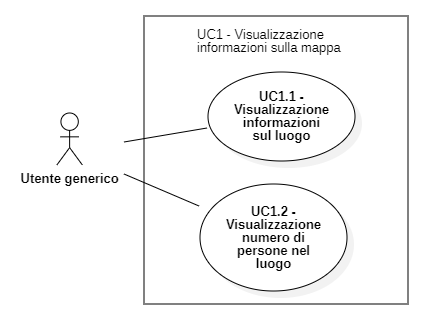
\includegraphics[scale=0.8]{../immagini/attori_casi/UC1_1_2.png}
		\caption{Schema sotto-casi d'uso visualizzazione informazioni della mappa}
	\end{figure}
\end{center}


\begin{itemize}
	\item \textbf{Attori primari}: utente generico;
	\item \textbf{Descrizione}: l’utente accede all’applicazione web e visualizza la heat map$_{\scaleto{G}{3pt}}$. La mappa mostra la città impostata di default o quella selezionata tra quelle a disposizione, come definito nell’UC8(sezione \ref{CasiDUsoCasiDUsoTraUnUtenteEIlFrontEndElencoCasiDUsoUC4SelezioneCittaDaVisualizzareNellaMappa}). Le informazioni vengono ricavate dall’orario e dalla data impostate dall’utente come indicato nel UC9.1(sezione \ref{CasiDUsoCasiDUsoTraUnUtenteEIlFrontEndElencoCasiDUsoUC51SelezioneDellOrario}) e UC9.2(sezione
	\ref{CasiDUsoCasiDUsoTraUnUtenteEIlFrontEndElencoCasiDUsoUC52ModificaDellaData}) o si utilizzano i dati in tempo reale, quindi usando l’orario attuale;
	\item \textbf{Scenario principale}: L’utente accede all’applicazione web e visualizza la heat map$_{\scaleto{G}{3pt}}$. La mappa mostra la città impostata di default o quella selezionata tra quelle a disposizione, come definito nell’UC8(sezione \ref{CasiDUsoCasiDUsoTraUnUtenteEIlFrontEndElencoCasiDUsoUC4SelezioneCittaDaVisualizzareNellaMappa}). Le informazioni vengono ricavate dall’orario e dalla data impostate dall’utente come indicato nel UC9.1(sezione \ref{CasiDUsoCasiDUsoTraUnUtenteEIlFrontEndElencoCasiDUsoUC51SelezioneDellOrario}) e UC9.2(sezione \ref{CasiDUsoCasiDUsoTraUnUtenteEIlFrontEndElencoCasiDUsoUC52ModificaDellaData}) o si utilizzano i dati in tempo reale, quindi usando l’orario attuale;accede all’applicazione web e visualizza la heat map$_{\scaleto{G}{3pt}}$ della città;
	\item \textbf{Precondizione}: il front end$_{\scaleto{G}{3pt}}$ può generare la mappa; la città, la data, l’ora sono state indicate dall’utente, seguendo quanto descritto rispettivamente nell'UC8 (sezione \ref{CasiDUsoCasiDUsoTraUnUtenteEIlFrontEndElencoCasiDUsoUC4SelezioneCittaDaVisualizzareNellaMappa}), nell'UC9.2(sezione \ref{CasiDUsoCasiDUsoTraUnUtenteEIlFrontEndElencoCasiDUsoUC52ModificaDellaData}) e nell'UC9.1(sezione \ref{CasiDUsoCasiDUsoTraUnUtenteEIlFrontEndElencoCasiDUsoUC51SelezioneDellOrario}), o vengono utilizzate quelle di default, quindi data e ora sono quelle odierne di sistema per dati in tempo reale e la città è quella impostata di default;
	\item \textbf{Postcondizione}: l’utente visualizza la heat map$_{\scaleto{G}{3pt}}$ con i dati ricavati nell’istante di tempo selezionato, come definito nell’UC9 (sezione \ref{CasiDUsoCasiDUsoTraUnUtenteEIlFrontEndElencoCasiDUsoUC5SelezioneDellIstanzeDiCuiVisualizzareIDatiNellaHeatmap}), e alla città scelta fra quelle disponibili come descritto nella definizione dell’UC8 (sezione \ref{CasiDUsoCasiDUsoTraUnUtenteEIlFrontEndElencoCasiDUsoUC4SelezioneCittaDaVisualizzareNellaMappa});
	\item \textbf{Estensioni}: l’utente accede all’applicazione web, il front end$_{\scaleto{G}{3pt}}$, rilevando la richiesta di generazione della mappa, individua una mancanza di dati per la sua costruzione e di conseguenza viene visualizzato un messaggio relativo all’errore riscontrato (UC2, sezione \ref{CasiDUsoCasiDUsoTraUnUtenteEIlFrontEndElencoCasiDUsoUC2VisualizzazioneMessaggioPerLaMancanzaDiDati});
\end{itemize}

\subsubsection{UC1.1 - Visualizzazione informazioni sul luogo }\label{CasiDUsoCasiDUsoTraUnUtenteEIlFrontEndElencoCasiDUsoUC1.1VisualizzazioneInformazioniSulLuogo} %parzialmente corretto
%ci penso
\begin{itemize}
	\item \textbf{Attori primari}: utente generico;
	\item \textbf{Descrizione}: l'utente visualizza le informazioni riguardanti il luogo specifico nella città visualizzata;
	\item \textbf{Scenario principale}:  l'utente attraverso la mappa visualizza il luogo specifico dove è situata la telecamera e attraverso l'UC7 (sezione \ref{CasiDUsoCasiDUsoTraUnUtenteEIlFrontEndElencoCasiDUsoUC312VisualizzazioneDelPopupDiUnPuntoDiInteresse}) può leggere la posizione precisa;%ci penso 
	\item \textbf{Precondizione}: il front end$_{\scaleto{G}{3pt}}$ può generare la mappa, la città è stata indicata dall’utente,, seguendo quanto descritto rispettivamente nell'UC8 (sezione \ref{CasiDUsoCasiDUsoTraUnUtenteEIlFrontEndElencoCasiDUsoUC4SelezioneCittaDaVisualizzareNellaMappa}), o è quella di default;
	\item \textbf{Postcondizione}: l’utente visualizza le informazioni della locazione in cui è posizionata la telecamera nella città;
\end{itemize}

\subsubsection{UC1.2 - Visualizzazione numero persone nel luogo }\label{CasiDUsoCasiDUsoTraUnUtenteEIlFrontEndElencoCasiDUsoUC1.2VisualizzazioneNumeroPersoneNelLuogo} %parzialmente corretto

\begin{itemize}
	\item \textbf{Attori primari}: utente generico;
	\item \textbf{Descrizione}: l'utente visualizza le informazioni riguardanti il numero di persone specifico della zona della città visualizzata;
	\item \textbf{Scenario principale}: l'utente attraverso la mappa visualizza il numero di persone presenti nel luogo rilevato dalla telecamera, si può visualizzare attraverso il colore della mappa o dall'UC7 (sezione \ref{CasiDUsoCasiDUsoTraUnUtenteEIlFrontEndElencoCasiDUsoUC312VisualizzazioneDelPopupDiUnPuntoDiInteresse});
	\item \textbf{Precondizione}: il front-end$_{\scaleto{G}{3pt}}$ genera la mappa e le informazioni relative al numero di persone per il luogo visualizzato sono presenti nel database; %ci penso
	\item \textbf{Postcondizione}: l’utente visualizza le informazioni del numero di persone in cui è posizionata la telecamera nella città;
\end{itemize}


\subsubsection{UC2 - Visualizzazione messaggio per la mancanza di informazioni }\label{CasiDUsoCasiDUsoTraUnUtenteEIlFrontEndElencoCasiDUsoUC2VisualizzazioneMessaggioPerLaMancanzaDiDati} %parzialmente corretto
\begin{itemize}
	\item \textbf{Attori primari}: utente generico;
	\item \textbf{Descrizione}: l’utente visualizza un'errore per la mancanza di dati necessari alla generazione della mappa. Questo accade quando il front end$_{\scaleto{G}{3pt}}$ non ha a disposizione tutti i dati;
	\item \textbf{Scenario principale}:
	\begin{itemize}
		\item l’operazione di generazione della mappa fallisce;
		\item l’utente visualizza un errore per la mancanza dei dati;
		\item l’utente clicca il pulsante “ok” per chiudere il messaggio.
	\end{itemize}
	\item \textbf{Precondizione}: il front end$_{\scaleto{G}{3pt}}$ effettua un controllo sui dati, non sono presenti tutti i dati;
	\item \textbf{Postcondizione}: viene mostrato un messaggio all’utente per informarlo sul problema riscontrato e l’operazione fallisce.
\end{itemize}



\subsubsection{UC29 - Spostamento all'interno della mappa}\label{CasiDUsoCasiDUsoTraUnUtenteEIlFrontEndElencoCasiDUsoUC29InterazioneConLaMappa} %ci penso inserisci la png UC29 chiamata UC3-4-5-8-9 in starUMl
\begin{center}
	\begin{figure}[H]
		\centering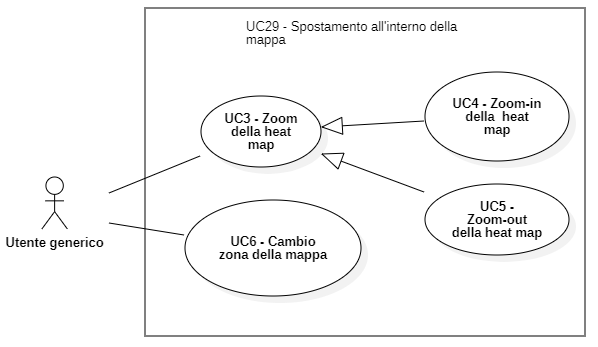
\includegraphics[scale=0.8]{../immagini/attori_casi/UC29.png}
		\caption{Schema generale spostamento all'interno della mappa}
	\end{figure}
\end{center}

\begin{itemize}
	\item \textbf{Attori primari}: utente generico;
	\item \textbf{Descrizione}: l’utente attraverso l'interfaccia dell'applicazione può interagire con la mappa spostandosi al suo interno;
	\item \textbf{Scenario principale}: l'utente può compiere diverse azioni nella mappa:
	\begin{itemize}
		\item Zoom della heat map, (sezione \ref{CasiDUsoCasiDUsoTraUnUtenteEIlFrontEndElencoCasiDUsoUC3ZoomDellaHeatMap}) ;
		\item Cambio zona della mappa, (sezione \ref{CasiDUsoCasiDUsoTraUnUtenteEIlFrontEndElencoCasiDUsoUC311SpostamentoDelCentroDellaMappa}).
	\end{itemize}
	\item \textbf{Precondizione}: la heat map è stata caricata correttamente;
	\item \textbf{Postcondizione}: l'utente interagendo con la mappa ne modifica lo zoom o il centro di visualizzazione.
\end{itemize}

\subsubsection{UC3 - Zoom della heat map}\label{CasiDUsoCasiDUsoTraUnUtenteEIlFrontEndElencoCasiDUsoUC3ZoomDellaHeatMap}

Dopo un'attenta analisi, il gruppo ha deciso di porre questo caso d'uso separato rispetto all'UC1 (sezione \ref{CasiDUsoCasiDUsoTraUnUtenteEIlFrontEndElencoCasiDUsoUC1VisualizzazioneInformazioniSullaMappa}) con lo scopo di renderlo disponibile per una possibile mappa differente da quella presente.

\begin{itemize}
	\item \textbf{Attori primari:} utente generico;
	\item \textbf{Descrizione:} l’utente, durante la visualizzazione della heat map$_{\scaleto{G}{3pt}}$, può variare il livello di zoom della mappa della città selezionata attraverso l'interfaccia;
	\item \textbf{Scenario principale:} l’utente attraverso l'interfaccia può decidere di modificare il livello di zoom della mappa visualizzata;
	\item \textbf{Generalizzazioni:}\begin{enumerate}
		\item UC4 - Zoom-in della heat map$_{\scaleto{G}{3pt}}$;
		\item UC5 - Zoom-out della heat map$_{\scaleto{G}{3pt}}$.
	\end{enumerate}
	\item \textbf{Precondizione:} il sistema è funzionante e la mappa è stata caricata;
	\item \textbf{Postcondizione:} il livello di zoom della mappa è aumentato o diminuito in base all'azione che compie l'utente.
\end{itemize}

\subsubsection{UC4 - Zoom-in della heat map}\label{CasiDUsoCasiDUsoTraUnUtenteEIlFrontEndElencoCasiDUsoUC31ZoomInDellaHeatMap}

\begin{itemize}
	\item \textbf{Attori primari:} utente generico;
	\item \textbf{Descrizione:} l’utente, durante la visualizzazione della heat map$_{\scaleto{G}{3pt}}$, può aumentare il livello di zoom per vedere in dettaglio la mappa della città selezionata;
	\item \textbf{Scenario principale:} l’utente aumenta il livello di zoom della heat map$_{\scaleto{G}{3pt}}$ per una visualizzazione più dettagliata della città. Dopo aver compiuto questa azione, l'utente inoltre, può spostarsi all'interno della mappa (UC6, sezione \ref{CasiDUsoCasiDUsoTraUnUtenteEIlFrontEndElencoCasiDUsoUC311SpostamentoDelCentroDellaMappa}) e visualizzare le etichette (denonimate pop-up$_G$) dei punti di interesse (UC7, sezione \ref{CasiDUsoCasiDUsoTraUnUtenteEIlFrontEndElencoCasiDUsoUC312VisualizzazioneDelPopupDiUnPuntoDiInteresse});
	\item \textbf{Precondizione:} il sistema dispone di informazioni relative alla città e il livello di zoom-in non è al massimo;
	\item \textbf{Postcondizione:} la heat map$_{\scaleto{G}{3pt}}$ si aggiorna mostrando livelli di informazioni più dettagliate in base al livello di zoom in effettuato.
\end{itemize}

\subsubsection{UC5 - Zoom-out della heat map}\label{CasiDUsoCasiDUsoTraUnUtenteEIlFrontEndElencoCasiDUsoUC32ZoomOutDellaHeatMap}

\begin{itemize}
	\item \textbf{Attori primari:} utente generico;
	\item \textbf{Descrizione:} l’utente, durante la visualizzazione della heat map$_{\scaleto{G}{3pt}}$, può diminuire il livello di zoom per vedere informazioni meno dettagliate della città selezionata;
	\item \textbf{Scenario principale:} l’utente diminuisce il livello di zoom della heat map$_{\scaleto{G}{3pt}}$ per una visualizzazione meno dettagliata della città;
	\item \textbf{Precondizione:}  il sistema dispone di informazioni relative alla città e il livello di zoom-out non è al massimo;
	\item \textbf{Postcondizione:} la heat map$_{\scaleto{G}{3pt}}$ si aggiorna mostrando livelli di informazioni meno dettagliate in base al livello di zoom-out effettuato.
\end{itemize}

\subsubsection{UC6 - Cambio zona della mappa}\label{CasiDUsoCasiDUsoTraUnUtenteEIlFrontEndElencoCasiDUsoUC311SpostamentoDelCentroDellaMappa}

\begin{itemize}
	\item \textbf{Attori primari:} utente generico;
	\item \textbf{Descrizione:} l’utente può spostarsi all’interno della mappa, infatti, utilizzando il cursore, può trascinare la mappa nel punto che vuole visualizzare;
	\item \textbf{Scenario principale:} l'utente decide di visualizzare un punto diverso da quello di default, presentato nella mappa, e quindi, trascinandola, si sposta per osservarlo;
	\item \textbf{Precondizione:} l'utente sta visualizzando la mappa nelle coordinate della città scelta o impostasta di default;
	\item \textbf{Postcondizione:} visualizza la mappa in un punto diverso rispetto al punto di partenza.
\end{itemize}


\subsubsection{UC7 - Visualizzazione delle informazioni nell'etichetta del punto di interesse}\label{CasiDUsoCasiDUsoTraUnUtenteEIlFrontEndElencoCasiDUsoUC312VisualizzazioneDelPopupDiUnPuntoDiInteresse}

\begin{itemize}
	\item \textbf{Attori primari:} utente generico;
	\item \textbf{Descrizione:} l’utente visualizza un'icona del punto di interesse. All'icona è associata un'etichetta contenente le informazioni riguardanti ad essa;
	\item \textbf{Scenario principale:} l’utente ha effettuato uno o più zoom-in sulla zona di interesse e visualizza l'etichetta informativa riferita alla città. L'utente può decidere di chiudere l'etichetta;
	\item \textbf{Precondizione:} il livello di zoom-in è maggiore di quello iniziale ed il sistema dispone delle informazioni da visualizzare nell'etichetta;
	\item \textbf{Postcondizione:} l’utente visualizza l'etichetta.
\end{itemize}

\subsubsection{UC8 - Selezione città da visualizzare nella mappa}\label{CasiDUsoCasiDUsoTraUnUtenteEIlFrontEndElencoCasiDUsoUC4SelezioneCittaDaVisualizzareNellaMappa}

\begin{itemize}
	\item \textbf{Attori primari}: utente generico;
	\item \textbf{Descrizione}: l’utente può selezionare la città di cui vuole visualizzare la heat map$_{\scaleto{G}{3pt}}$;
	\item \textbf{Scenario principale}: l’utente seleziona una città tra quelle messe a disposizione;
	\item \textbf{Precondizione}: il sistema dispone di informazioni relative a diverse città;
	\item \textbf{Postcondizione}:  l’utente ha selezionato la città che vuole visualizzare, la heat-map$_{\scaleto{G}{3pt}}$ si aggiorna in base alla scelta fatta.
\end{itemize}

\subsubsection{UC9 - Selezione dell’istante di cui visualizzare i dati nella heat map
}\label{CasiDUsoCasiDUsoTraUnUtenteEIlFrontEndElencoCasiDUsoUC5SelezioneDellIstanzeDiCuiVisualizzareIDatiNellaHeatmap}%parzialmente corretto
\begin{center}
	\begin{figure}[H]
		\centering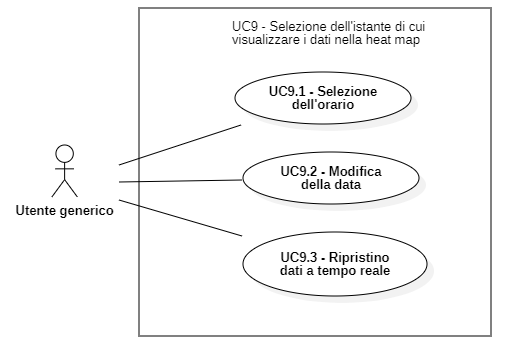
\includegraphics[scale=0.7]{../immagini/attori_casi/UC_9_1_2_3.png}
		\caption{Schema sotto-casi della selezione dell'istante da visualizzare}
	\end{figure}
\end{center}
\begin{itemize}
	\item \textbf{Attori primari}: utente generico;
	\item \textbf{Descrizione}: l’utente, attraverso l’interfaccia del sistema, modifica l’istante di tempo di cui vuole visualizzare i dati;
	\item \textbf{Scenario principale}: attraverso l’interfaccia l’utente può decidere di:
		\begin{enumerate}
			\item Modificare l’orario dei dati da visualizzare (UC9.1, sezione  \ref{CasiDUsoCasiDUsoTraUnUtenteEIlFrontEndElencoCasiDUsoUC51SelezioneDellOrario});
			\item Modificare la data tra quelle disponibili (UC9.2, sezione \ref{CasiDUsoCasiDUsoTraUnUtenteEIlFrontEndElencoCasiDUsoUC52ModificaDellaData});
			\item Ritornare ai dati in tempo reale (UC9.3, sezione \ref{CasiDUsoCasiDUsoTraUnUtenteEIlFrontEndElencoCasiDUsoUC53RipristinoDatiATempoReale}).
		\end{enumerate}
	\item \textbf{Precondizione}: il sistema dispone di informazioni su diversi istanti di tempo;
	\item \textbf{Postcondizione}: l’utente ha selezionato un istante di tempo diverso da quello attuale e visualizza i dati riguardanti ad esso.%insicuro
\end{itemize}

\subsubsection{UC9.1 - Selezione dell’orario}\label{CasiDUsoCasiDUsoTraUnUtenteEIlFrontEndElencoCasiDUsoUC51SelezioneDellOrario}
\begin{itemize}
	\item \textbf{Attori primari}: utente generico;
	\item \textbf{Descrizione}: l’utente seleziona un orario diverso da quello attuale per visualizzare i dati di quel momento;
	\item \textbf{Scenario principale}: l’utente imposta un orario utilizzando l’interfaccia dell’applicazione web;
	\item \textbf{Precondizione}: il sistema ha informazioni riguardanti tutti i diversi orari; %insicuro
	\item \textbf{Postcondizione}: l’orario viene aggiornato e la mappa visualizza i dati della modifica fatta.
\end{itemize}

\subsubsection{UC9.2 - Modifica della data}\label{CasiDUsoCasiDUsoTraUnUtenteEIlFrontEndElencoCasiDUsoUC52ModificaDellaData}
\begin{itemize}
	\item \textbf{Attori primari}: utente generico;
	\item \textbf{Descrizione}: l’utente seleziona una data diversa da quella odierna tra quelle disponibili e visualizza la mappa della data scelta;
	\item \textbf{Scenario principale}: l’utente seleziona una data diversa da quella attuale;
	\item \textbf{Precondizione}: il sistema possiede informazioni su tutte le date fino a quella odierna;
	\item \textbf{Postcondizione}: la data viene aggiornata e l’utente visualizza l’heat map$_{\scaleto{G}{3pt}}$ aggiornata con i dati del giorno selezionato all’orario attuale o all’orario scelto dall’utente stesso, secondo quanto definito nella descrizione dell’UC9.1 (sezione \ref{CasiDUsoCasiDUsoTraUnUtenteEIlFrontEndElencoCasiDUsoUC51SelezioneDellOrario}).
\end{itemize}

\subsubsection{UC9.3 - Ripristino dati a tempo reale}\label{CasiDUsoCasiDUsoTraUnUtenteEIlFrontEndElencoCasiDUsoUC53RipristinoDatiATempoReale}
\begin{itemize}
	\item \textbf{Attori primari}: utente generico;
	\item \textbf{Descrizione}: l’utente sceglie di osservare i dati in tempo reale;
	\item \textbf{Scenario principale}: l’utente preme sul pulsante per il ripristino dei valori attuali di data e ora;
	\item \textbf{Precondizione}: l’utente ha impostato una data e/o un’ora diversa dal valore di quella attuale secondo quanto descritto nell'UC9.1 (sezione \ref{CasiDUsoCasiDUsoTraUnUtenteEIlFrontEndElencoCasiDUsoUC51SelezioneDellOrario}) e nell'UC9.2 (sezione \ref{CasiDUsoCasiDUsoTraUnUtenteEIlFrontEndElencoCasiDUsoUC52ModificaDellaData});
	\item \textbf{Postcondizione}: l’utente visualizza la mappa con i dati in tempo reale.
\end{itemize}


\begin{center}
	\begin{figure}[H]
		\centering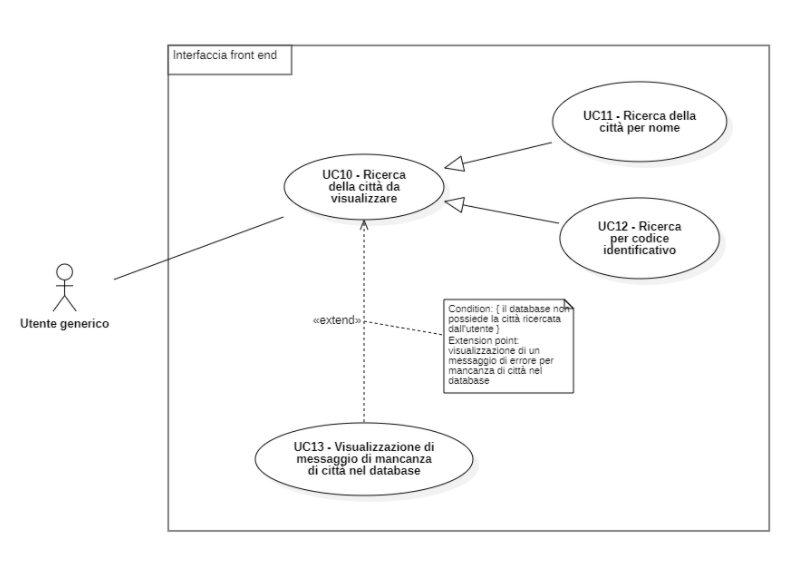
\includegraphics[scale=0.6]{../immagini/attori_casi/UC_10.png}
		\caption{Scherma generale della ricerca ed errori annessi}
	\end{figure}
\end{center}


\subsubsection{UC10 - Ricerca della città da visualizzare}\label{CasiDUsoCasiDUsoTraUnUtenteEIlFrontEndElencoCasiDUsoUC6RicercaDellaCittàDaVisualizzare}

\begin{itemize}
	\item \textbf{Attori primari:} utente generico;
	\item \textbf{Descrizione:} l’utente può ricercare, in una barra di ricerca, la città da visualizzare;
	\item \textbf{Scenario principale:} l’utente ricerca una città tramite una barra di ricerca;
	\item \textbf{Precondizione:} l’utente ha inserito la città da ricercare;
	\item \textbf{Postcondizione:} l’utente ha inserito la città che vuole cercare e il sistema si aggiorna in base alla ricerca fatta;
	\item \textbf{Generalizzazioni:}
	\begin{itemize}
		\item ricerca della città tramite il suo nome UC11 (sezione \ref{CasiDUsoCasiDUsoTraUnUtenteEIlFrontEndElencoCasiDUsoUC52RicercaDellaCittàDaVisualizzareTramiteNome});
		\item ricerca della città tramite il suo codice UC12 (sezione \ref{CasiDUsoCasiDUsoTraUnUtenteEIlFrontEndElencoCasiDUsoUC61RicercaDellaCittàDaVisualizzareTramiteCodiceIdentificativo}).
	\end{itemize}
	\item \textbf{Estensioni:} l’utente ha ricercato una città non presente nel database, il sistema rileva questo errore e di conseguenza viene visualizzato un messaggio relativo all’errore riscontrato (UC13, sezione \ref{CasiDUsoCasiDUsoTraUnUtenteEIlFrontEndElencoCasiDUsoUC7VisualizzazioneMessaggioDiMancanzaCittàNelDatabase}).
\end{itemize}


\subsubsection{UC11 - Ricerca della città per nome}\label{CasiDUsoCasiDUsoTraUnUtenteEIlFrontEndElencoCasiDUsoUC52RicercaDellaCittàDaVisualizzareTramiteNome}

\begin{itemize}
	\item \textbf{Attori primari:} utente generico;
	\item \textbf{Descrizione:} l’utente ha la possibilità di ricercare la città da visualizzare tramite nome;
	\item \textbf{Scenario principale:} l’utente ricerca la città tramite nome;
	\item \textbf{Precondizione:} l’utente ha inserito il nome della città da ricercare;
	\item \textbf{Postcondizione:} il sistema mostra all’utente il risultato della ricerca effettuata.
\end{itemize}

\subsubsection{UC12 - Ricerca della città per codice identificativo}\label{CasiDUsoCasiDUsoTraUnUtenteEIlFrontEndElencoCasiDUsoUC61RicercaDellaCittàDaVisualizzareTramiteCodiceIdentificativo}
\begin{itemize}
	\item \textbf{Attori primari:} utente generico;
	\item \textbf{Descrizione:} l’utente ha la possibilità di ricercare la città da visualizzare tramite codice identificativo;
	\item \textbf{Scenario principale:} l’utente ricerca la città tramite codice identificativo;
	\item \textbf{Precondizione:} l’utente ha inserito il codice identificativo della città da ricercare;
	\item \textbf{Postcondizione:} il sistema mostra all’utente il risultato della ricerca effettuata.
\end{itemize}



\subsubsection{UC13 - Visualizzazione mancanza città nel database}\label{CasiDUsoCasiDUsoTraUnUtenteEIlFrontEndElencoCasiDUsoUC7VisualizzazioneMessaggioDiMancanzaCittàNelDatabase}

\begin{itemize}
	\item \textbf{Attori primari:} utente generico;
	\item \textbf{Descrizione:} l’utente visualizza un errore per l'inserimento nella barra di ricerca di una città non presente nel database;
	\item \textbf{Scenario principale:}
	\begin{enumerate}
		\item l’operazione di ricerca fallisce;
		\item l’utente visualizza un errore;
		\item l’utente preme "ok" per chiudere il messaggio.
	\end{enumerate}
	\item \textbf{Precondizione:} il front end$_{\scaleto{G}{3pt}}$ effettua un controllo sui dati e non è presente la città ricercata;
	\item \textbf{Postcondizione:} viene visualizzato  un messaggio all’utente per informarlo sul problema.
\end{itemize}

\section{Casi d'uso tra il front end e il back end}\label{CasiDUsoCasiDUsoTraIlFrontEndEIlBackEnd}
%spiegazione sezione

\subsection{Attori dei casi d'uso}\label{CasiDUsoCasiDUsoTraIlFrontEndEIlBackEndAttoriDeiCasiDUso}
%immagine errata
\begin{center}
	\begin{figure}[H]
		\centering
\includegraphics{../immagini/attori_casi/sistema_front_end.png}
		\caption{Attore: Sistema front end}
	\end{figure}
\end{center}
\subsubsection{Attori Primari}\label{CasiDUsoCasiDUsoTraIlFrontEndEIlBackEndAttoriDeiCasiDUsoAttoriPrimari}
\begin{itemize}
	\item \textbf{Sistema front end$_{\scaleto{G}{3pt}}$:} Definisce una parte del sistema sviluppato che interagisce con il sistema back end$_{\scaleto{G}{3pt}}$.
\end{itemize}

\subsection{Elenco casi d'uso}\label{CasiDUsoCasiDUsoTraIlFrontEndEIlBackEndElencoDeiCasiDUso}

\subsubsection{UC14 - Visualizzazione dei dati di uno specifico istante passato}\label{CasiDUsoCasiDUsoTraIlFrontEndEIlBackEndElencoDeiCasiDUsoUC81VisualizzazioneDeiDatiDiUnoSpecificoIstante}
\begin{itemize}
	\item \textbf{Attori primari}: sistema front end$_{\scaleto{G}{3pt}}$;
	\item \textbf{Descrizione}: il front end$_{\scaleto{G}{3pt}}$ richiede le informazioni relative ad uno specifico istante di tempo passato, vengono visualizzate le informazioni inviate dal back end$_{\scaleto{G}{3pt}}$;
	\item \textbf{Scenario principale}:  il front end$_{\scaleto{G}{3pt}}$ richiede al back end$_{\scaleto{G}{3pt}}$ le informazioni relative all'istante di tempo passato specificato, il back end$_{\scaleto{G}{3pt}}$ invia le informazioni da visualizzare al front end$_{\scaleto{G}{3pt}}$;
	\item \textbf{Precondizione}: l’utente esegue la modifica della data o dell’orario come definito rispettivamente nella descrizione di UC9.2 (sezione \ref{CasiDUsoCasiDUsoTraUnUtenteEIlFrontEndElencoCasiDUsoUC52ModificaDellaData}) e UC9.1 (sezione \ref{CasiDUsoCasiDUsoTraUnUtenteEIlFrontEndElencoCasiDUsoUC51SelezioneDellOrario}) selezionando un istante di tempo precedente a quello attuale;
	\item \textbf{Postcondizione}: il front end$_{\scaleto{G}{3pt}}$ visualizza e riceve le informazioni relative all'istante di tempo passato impostato;
	\item \textbf{Estensione}: il front end$_{\scaleto{G}{3pt}}$ effettua la richiesta al back end$_{\scaleto{G}{3pt}}$ il quale non invia nessun dato nella risposta (UC17, sezione \ref{CasiDUsoCasiDUsoTraIlFrontEndEIlBackEndElencoDeiCasiDUsoUC9VisualizzazioneMessaggioDiMancanzaDatiDalBackEnd}).
\end{itemize}


\subsubsection{UC15 - Visualizzazione dei dati in tempo reale}\label{CasiDUsoCasiDUsoTraIlFrontEndEIlBackEndElencoDeiCasiDUsoUC82VisualizzazioneDeiDatiInTempoReale}
\begin{itemize}
	\item \textbf{Attori primari}: sistema front end$_{\scaleto{G}{3pt}}$;
	\item \textbf{Descrizione}: il front end$_{\scaleto{G}{3pt}}$ visualizza i dati reali più recentemente aggiunti;
	\item \textbf{Scenario principale}: il front end$_{\scaleto{G}{3pt}}$ richiede al back end$_{\scaleto{G}{3pt}}$ le informazioni più recentemente aggiunte, una volta ricevute il front end$_{\scaleto{G}{3pt}}$ le visualizza;
	\item \textbf{Precondizione}: viene eseguita la visualizzazione della mappa come definito nell’UC1 (sezione \ref{CasiDUsoCasiDUsoTraUnUtenteEIlFrontEndElencoCasiDUsoUC1VisualizzazioneInformazioniSullaMappa}) o avviene il ripristino dei dati in tempo reale come definito in UC9.3 (sezione \ref{CasiDUsoCasiDUsoTraUnUtenteEIlFrontEndElencoCasiDUsoUC53RipristinoDatiATempoReale});
	\item \textbf{Postcondizione}: il front end$_{\scaleto{G}{3pt}}$ ha ricevuto e visualizzato i dati ed è pronto alla generazione della heat map$_{\scaleto{G}{3pt}}$;
	\item \textbf{Estensione}: il front end$_{\scaleto{G}{3pt}}$ effettua la richiesta al back end$_{\scaleto{G}{3pt}}$ il quale non invia nessun dato nella risposta (UC17, sezione \ref{CasiDUsoCasiDUsoTraIlFrontEndEIlBackEndElencoDeiCasiDUsoUC9VisualizzazioneMessaggioDiMancanzaDatiDalBackEnd}).
\end{itemize}

\subsubsection{UC16 - Visualizzazione dei dati futuri predetti}\label{CasiDUsoCasiDUsoTraIlFrontEndEIlBackEndElencoDeiCasiDUsoUC83VisualizzazioneDeiDatiPredetti}
\begin{itemize}
	\item \textbf{Attori primari}: sistema front end$_{\scaleto{G}{3pt}}$;
	\item \textbf{Descrizione}: il front end$_{\scaleto{G}{3pt}}$ richiede i dati i dati della previsione fino al giorno seguente.
	I dati sono ricavati dall’elaborazione, attraverso un modello di machine learning$_{\scaleto{G}{3pt}}$, dei dati reali acquisti. Una volta ricevuti i dati, il front end$_{\scaleto{G}{3pt}}$ li può visualizzare;
	\item \textbf{Scenario principale}: il front end$_{\scaleto{G}{3pt}}$ richiede al back end$_{\scaleto{G}{3pt}}$ i dati elaborati dal modello machine learning$_{\scaleto{G}{3pt}}$. Completata la richiesta il front end$_{\scaleto{G}{3pt}}$ visualizzerà i dati inviati dal back end$_{\scaleto{G}{3pt}}$;
	\item \textbf{Precondizione}: le informazioni vengono visualizzate sulla mappa come definito nell’UC1 (sezione \ref{CasiDUsoCasiDUsoTraUnUtenteEIlFrontEndElencoCasiDUsoUC1VisualizzazioneInformazioniSullaMappa}), impostando un orario successivo a quello attuale come descritto nell’UC9.1 (sezione \ref{CasiDUsoCasiDUsoTraUnUtenteEIlFrontEndElencoCasiDUsoUC51SelezioneDellOrario});
	\item \textbf{Postcondizione}: il front end$_{\scaleto{G}{3pt}}$ ha ricevuto e visualizzato i dati ed è pronto alla generazione della heat map$_{\scaleto{G}{3pt}}$;
	\item \textbf{Estensione}: il front end$_{\scaleto{G}{3pt}}$ effettua la richiesta al back end$_{\scaleto{G}{3pt}}$ il quale non invia nessun dato nella risposta (UC17, sezione \ref{CasiDUsoCasiDUsoTraIlFrontEndEIlBackEndElencoDeiCasiDUsoUC9VisualizzazioneMessaggioDiMancanzaDatiDalBackEnd}).
\end{itemize}

\subsubsection{UC17 - Visualizzazione mancanza dati dal back end}\label{CasiDUsoCasiDUsoTraIlFrontEndEIlBackEndElencoDeiCasiDUsoUC9VisualizzazioneMessaggioDiMancanzaDatiDalBackEnd}
\begin{itemize}
	\item \textbf{Attori primari}: sistema front end$_{\scaleto{G}{3pt}}$;
	\item \textbf{Descrizione}: il front end$_{\scaleto{G}{3pt}}$ riceve un errore per la mancanza dati rispetto alla richiesta di visualizzazione effettuata;
	\item \textbf{Scenario principale}:
	\begin{enumerate}
		\item il front end$_{\scaleto{G}{3pt}}$ richiede dei dati specifici al back end$_{\scaleto{G}{3pt}}$;
		\item la risposta ricevuta è un errore;
		\item il front end$_{\scaleto{G}{3pt}}$ ritenta la richiesta di informazioni.
	\end{enumerate}
	\item \textbf{Precondizione}: il front end$_{\scaleto{G}{3pt}}$ effettua una richiesta di dati, il back end$_{\scaleto{G}{3pt}}$ non ha a disposizione i dati richiesti;
	\item \textbf{Postcondizione}: il front end$_{\scaleto{G}{3pt}}$ riceve un errore per la mancanza dei dati da visualizzare.
\end{itemize}

\newpage
\section{Casi d'uso facoltativi tra un utente e il front end}\label{CasiDUsoCasiDUsoFacoltativiTraUnUtenteEIlFrontEnd}
%spiegazione della sezione
L'elenco dei casi d'uso in questa sezione individuano requisiti sviluppabili successivamente a quelli obbligatori descritti nelle sezioni precedenti.
\subsection{Attori dei casi d'uso}
\begin{center}
	\begin{figure}[H]
		\centering
\includegraphics{../immagini/attori_casi/utente_generico.png}
		\caption{Attore: utente generico}
	\end{figure}
\end{center}
\subsubsection{Attori Primari}\label{UFattoriPrimariFac}
\begin{itemize}
	\item \textbf{Utente generico:} definisce l'utente generico che utilizza l'applicazione web.
\end{itemize}

\subsection{Elenco casi d'uso}\label{CasiDUsoCasiDUsoFacoltativiTraUnUtenteEIlFrontEndElencoCasiDUso}

\subsubsection{UC18 - Visualizzazione indici di affidabilità}\label{CasiDUsoCasiDUsoFacoltativiTraUnUtenteEIlFrontEndElencoCasiDUsoUC10VisualizzazioneIndiciDiAffidabilita}


\begin{itemize}
	\item \textbf{Attori primari}: utente generico;
	\item \textbf{Descrizione}: l'utente può visualizzare gli indici di affidabilità dei dati reali raccolti e l'indice di affidabilità delle predizioni svolte dal modello di machine learning$_{\scaleto{G}{3pt}}$;
	\item \textbf{Scenario principale}: l'utente attraverso l'interfaccia visualizza gli indici di affidabilità;
	\item \textbf{Precondizione}: il front end$_{\scaleto{G}{3pt}}$ dispone degli indici relativi ai dati reali e predetti;
	\item \textbf{Postcondizione}: l'utente visualizza correttamente gli indici di affidabilità dei dati reali e predetti.
\end{itemize}

\subsubsection{UC19 - Impostazioni avanzate sui dati}\label{CasiDUsoCasiDUsoFacoltativiTraUnUtenteEIlFrontEndElencoCasiDUsoUC11ImpostazioniAvanzateSuiDati}

\begin{center}
	\begin{figure}[H]
		\centering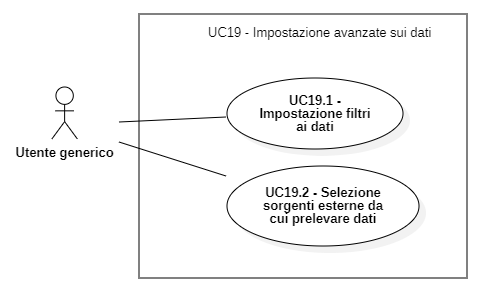
\includegraphics[scale=0.7]{../immagini/attori_casi/UC_19_1_2.png}
		\caption{Schema sotto-casi delle impostazioni avanzate sui dati}
	\end{figure}
\end{center}

\begin{itemize}
	\item \textbf{Attori primari}: utente generico;
	\item \textbf{Descrizione}: l'utente attraverso l'interfaccia del front end$_{\scaleto{G}{3pt}}$ può applicare filtri sui dati e modificare le sorgenti esterne da cui vengono prelevate le informazioni;
	\item \textbf{Scenario principale}: attraverso l'interfaccia l'utente può:
	\begin{itemize}
		\item Applicare filtri ai dati (UC19.1, sezione  \ref{CasiDUsoCasiDUsoFacoltativiTraUnUtenteEIlFrontEndElencoCasiDUsoUC111ApplicazioneFiltriAiDati});
		\item Modificare le sorgenti esterne da cui vengono prelevate le informazioni (UC19.2, sezione \ref{CasiDUsoCasiDUsoFacoltativiTraUnUtenteEIlFrontEndElencoCasiDUsoUC112SelezioneSorgentiEsterneDaCuiPrelevareIDati}).
	\end{itemize}
	\item \textbf{Precondizione}: l'utente visualizza correttamente l'interfaccia e sono disponibili varie sorgenti esterne;
	\item \textbf{Postcondizione}: l'utente applica le impostazioni scelte ai dati e viene aggiornata la mappa di conseguenza.
\end{itemize}

\subsubsection{UC19.1 - Applicazione filtri ai dati}\label{CasiDUsoCasiDUsoFacoltativiTraUnUtenteEIlFrontEndElencoCasiDUsoUC111ApplicazioneFiltriAiDati}
\begin{itemize}
	\item \textbf{Attori primari}: utente generico;
	\item \textbf{Descrizione}: l'utente attraverso l'interfaccia del front end$_{\scaleto{G}{3pt}}$ può applicare filtri sui dati reali e su quelli predetti, modificandone i colori con cui vengono visualizzati nella mappa;
	\item \textbf{Scenario principale}:
	\begin{enumerate}
		\item L'utente può selezionare il colore per i dati reali e/o per quelli predetti;
		\item L'utente conferma i filtri da applicare alla mappa.
	\end{enumerate}
	\item \textbf{Precondizione}: l'utente visualizza correttamente l'interfaccia;
	\item \textbf{Postcondizione}: l'utente applica i filtri ai dati e la mappa viene aggiornata di conseguenza.
\end{itemize}

\subsubsection{UC19.2 - Selezione sorgenti esterne da cui prelevare i dati}\label{CasiDUsoCasiDUsoFacoltativiTraUnUtenteEIlFrontEndElencoCasiDUsoUC112SelezioneSorgentiEsterneDaCuiPrelevareIDati}
\begin{itemize}
	\item \textbf{Attori primari}: utente generico;
	\item \textbf{Descrizione}: l'utente attraverso l'interfaccia del front end$_{\scaleto{G}{3pt}}$ dispone di un menù in cui può selezionare le sorgenti che vuole utilizzare per il reperimento dei dati;
	\item \textbf{Scenario principale}: l'utente decide di selezionare delle diverse sorgenti esterne e indica quelle da cui vuole prelevare informazioni;
	\item \textbf{Precondizione}: l'utente visualizza correttamente l'interfaccia, sono disponibili varie sorgenti esterne;
	\item \textbf{Postcondizione}: l'utente visualizza la mappa con i soli dati delle sorgenti scelte.
\end{itemize}

\subsubsection{UC20 - Recupero manuale utente}\label{CasiDUsoCasiDUsoFacoltativiTraUnUtenteEIlFrontEndElencoCasiDUsoUC12RecuperoManualeUtente}


\begin{itemize}
	\item \textbf{Attori primari}: utente generico;
	\item \textbf{Descrizione}: l'utente attraverso l'interfaccia del front end$_{\scaleto{G}{3pt}}$ può recuperare il manuale d'uso per informazioni sull'utilizzo dell'applicazione web;
	\item \textbf{Scenario principale}: l'utente seleziona il link al recupero del manuale utente;
	\item \textbf{Precondizione}: il front end$_{\scaleto{G}{3pt}}$ dispone del manuale utente;
	\item \textbf{Postcondizione}: l'utente dispone del manuale utente sul proprio dispositivo e lo può visualizzare.
\end{itemize}

\subsubsection{UC21 - Visualizzazione di dati a confronto di due città differenti}\label{CasiDUsoCasiDUsoFacoltativiTraUnUtenteEIlFrontEndElencoCasiDUsoUC13VisualizzazioneDiDatiAConfrontoDiDueCittaDifferenti}
\begin{center}
	\begin{figure}[H]
		\centering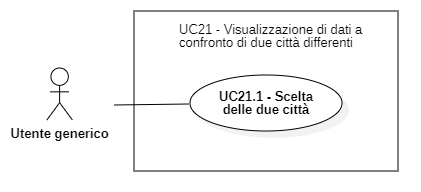
\includegraphics[scale=0.7]{../immagini/attori_casi/UC_21_1.png}
		\caption{Schema sotto-casi della visualizzazione delle città a confronto}
	\end{figure}
\end{center}

\begin{itemize}
	\item \textbf{Attori primari}: utente generico;
	\item \textbf{Descrizione}: l’utente può selezionare due città per poter mettere a confronto i loro dati;
	\item \textbf{Scenario principale}: l’utente seleziona le due città e visualizza i dati a confronto;
	\item \textbf{Precondizione}: il sistema dispone le informazioni riguardanti le città;
	\item \textbf{Postcondizione}: l'utente visualizza i dati di entrambe le città per poterli mettere a confronto.
\end{itemize}

\subsubsection{UC21.1 - Scelta delle due città}
\begin{itemize}
	\item \textbf{Attori primari}: utente generico;
	\item \textbf{Descrizione}: l'utente seleziona le due città da mettere a confronto per la visualizzazione dei dati;
	\item \textbf{Scenario principale}: l’utente seleziona le due città;
	\item \textbf{Precondizione}: il sistema ha informazioni su diverse città;
	\item \textbf{Postcondizione}: l'utente ha scelto le due città da confrontare.
\end{itemize}


\begin{center}
	\begin{figure}[H]
		\centering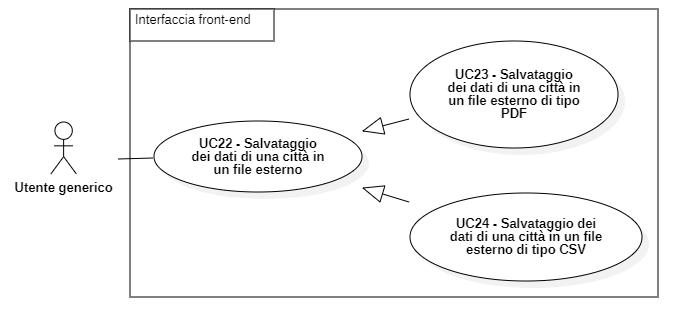
\includegraphics[scale=0.7]{../immagini/attori_casi/UC_22_23_24.png}
		\caption{Schema generale del salvataggio dei dati in un file esterno}
	\end{figure}
\end{center}


\subsubsection{UC22 - Salvataggio dei dati di una città in un file esterno}\label{CasiDUsoCasiDUsoFacoltativiTraUnUtenteEIlFrontEndElencoCasiDUsoUC14SalvataggioDeiDatiDiUnaCittaInUnFileEsterno}


\begin{itemize}
	\item \textbf{Attori primari}: utente generico;
	\item \textbf{Descrizione}: l’utente ha la possibilità di salvare localmente i dati relativi ad una città in un file;
	\item \textbf{Scenario principale}: l’utente salva localmente i dati della città che sta visualizzando;
	\item \textbf{Precondizione}: il sistema dispone delle informazioni riguardanti le città e  l’utente sta visualizzando la heat map$_{\scaleto{G}{3pt}}$ di una città in particolare;
	\item \textbf{Postcondizione}: il sistema ha salvato localmente i dati della città che sta visualizzando.
\end{itemize}

\subsubsection{UC23 - Salvataggio dei dati di una città in un file esterno di tipo PDF}\label{CasiDUsoCasiDUsoFacoltativiTraUnUtenteEIlFrontEndElencoCasiDUsoUC141SalvataggioDeiDatiDiUnaCittaInUnFileEsternoDiTipoPdf}

\begin{itemize}
	\item \textbf{Attori primari}: utente generico;
	\item \textbf{Descrizione}: l’utente può selezionare l’estensione del file in PDF;
	\item \textbf{Scenario principale}: l’utente seleziona l’estensione del file in PDF;
	\item \textbf{Precondizione}: il sistema dispone delle informazioni riguardanti le città e  l’utente sta visualizzando la heat map$_{\scaleto{G}{3pt}}$ di una città in particolare;
	\item \textbf{Postcondizione}: il sistema ha salvato localmente i dati in formato PDF.
\end{itemize}

\subsubsection{UC24 - Salvataggio dei dati di una città in un file esterno di tipo CSV}\label{CasiDUsoCasiDUsoFacoltativiTraUnUtenteEIlFrontEndElencoCasiDUsoUC142SalvataggioDeiDatiDiUnaCittaInUnFileEsternoDiTipoCsv}

\begin{itemize}
	\item \textbf{Attori primari}: utente generico;
	\item \textbf{Descrizione}: l’utente può selezionare l’estensione del file in CSV;
	\item \textbf{Scenario principale}: l’utente seleziona l’estensione del file in CSV;
	\item \textbf{Precondizione}: il sistema dispone delle informazioni riguardanti le città e  l’utente sta visualizzando la heat map$_{\scaleto{G}{3pt}}$ di una città in particolare;
	\item \textbf{Postcondizione}: il sistema ha salvato localmente i dati in formato CSV.
\end{itemize}

\subsubsection{UC25 - Scelta notifica via e-mail }\label{CasiDUsoCasiDUsoFacoltativiTraUnUtenteEIlFrontEndElencoCasiDUsoUC15NotificaViaEmailDiUnaCittaSelezionata}

\begin{center}
	\begin{figure}[H]
		\centering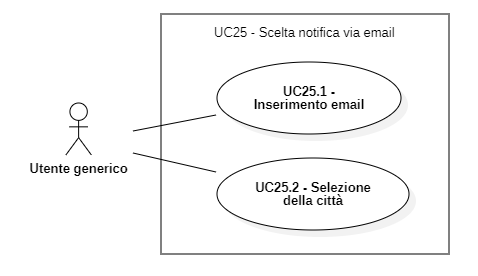
\includegraphics[scale=0.7]{../immagini/attori_casi/UC_25_1_2.png}
		\caption{Schema sotto-casi della scelta di notifica via e-mail}
	\end{figure}
\end{center}

\begin{itemize}
	\item \textbf{Attori primari}: utente generico;
	\item \textbf{Descrizione}: l'utente decide di voler essere notificato via e-mail riguardo gli aggiornamenti relativi ad una determinata città;
	\item \textbf{Scenario principale}:
		\begin{itemize}
			\item inserisce la propria mail (UC25.1, sezione \ref{CasiDUsoCasiDUsoFacoltativiTraUnUtenteEIlFrontEndElencoCasiDUsoUC15.1InserimentoEmail});
			\item seleziona la città di interesse (UC25.2, sezione \ref{CasiDUsoCasiDUsoFacoltativiTraUnUtenteEIlFrontEndElencoCasiDUsoUC15.2SelezioneCitta}).
		\end{itemize}
	\item \textbf{Precondizione}: l'utente sta visualizzando la heat map$_{\scaleto{G}{3pt}}$ e richiede la notifica via e-mail;
	\item \textbf{Postcondizione}: il sistema aggiunge nel database l'e-mail inserita dall'utente e la relativa città di interesse;
	\item \textbf{Estensioni}: il sistema determina che l'e-mail inserita non è valida, di conseguenza viene visualizzato un messaggio d'errore (UC26, sezione \ref{CasiDUsoCasiDUsoFacoltativiTraUnUtenteEIlFrontEndElencoCasiDUsoUC16VisualizzazioneMessaggioDiErroreEmailErrata}).
\end{itemize}

\subsubsection{UC25.1 - Inserimento email}\label{CasiDUsoCasiDUsoFacoltativiTraUnUtenteEIlFrontEndElencoCasiDUsoUC15.1InserimentoEmail}

\begin{itemize}
	\item \textbf{Attori primari}: utente generico;
	\item \textbf{Descrizione}: l'utente inserisce la propria email;
	\item \textbf{Scenario principale}: l'utente inserisce la propria email all'interno del form;
	\item \textbf{Precondizione}: l'utente ha richiesto la notificazione via email;
	\item \textbf{Postcondizione}: il sistema aggiunge nel database l'email inserita dall'utente.
\end{itemize}

\subsubsection{UC25.2 - Selezione della città}\label{CasiDUsoCasiDUsoFacoltativiTraUnUtenteEIlFrontEndElencoCasiDUsoUC15.2SelezioneCitta}

\begin{itemize}
	\item \textbf{Attori primari}: utente generico;
	\item \textbf{Descrizione}: l'utente seleziona la città di suo interesse;
	\item \textbf{Scenario principale}: l'utente seleziona la città di suo interesse;
	\item \textbf{Precondizione}: l'utente ha richiesto la notificazione via email;
	\item \textbf{Postcondizione}: il sistema aggiunge nel database la città selezionata dall'utente per ricevere le notifiche su di essa.
\end{itemize}


\subsubsection{UC26 - Visualizzazione messaggio di errore inserimento email}\label{CasiDUsoCasiDUsoFacoltativiTraUnUtenteEIlFrontEndElencoCasiDUsoUC16VisualizzazioneMessaggioDiErroreEmailErrata}

\begin{itemize}
	\item \textbf{Attori primari}: utente generico;
	\item \textbf{Descrizione}: Il front end$_{\scaleto{G}{3pt}}$ mostra a video un messaggio di errore nell'inserimento della email;
	\item \textbf{Scenario principale}: \begin{itemize}
		\item l'operazione di inserimento email fallisce;
		\item l'utente visualizza il messaggio d'errore;
		\item l'utente clicca il pulsante "ok" per chiudere il messaggio.
	\end{itemize}
	\item \textbf{Precondizione}: l'email inserita non è valida;
	\item \textbf{Postcondizione}: l'utente visualizza un messaggio di errore.
\end{itemize}

\subsubsection{UC27 - Visualizzazione lista delle città più cercate}\label{CasiDUsoCasiDUsoFacoltativiTraUnUtenteEIlFrontEndElencoCasiDUsoUC17VisualizzazioneListaDelleCittaPiuCercate}

\begin{itemize}
	\item \textbf{Attori primari}: utente generico;
	\item \textbf{Descrizione}: l'utente ha la possibilità di visionare la lista delle città più cercate all'interno del sito;
	\item \textbf{Scenario principale}: l'utente visualizza la lista;
	\item \textbf{Precondizione}: il sistema è funzionante e possiede le informazioni riguardanti le ricerche effettuate dagli utenti;
	\item \textbf{Postcondizione}: il back end$_{\scaleto{G}{3pt}}$ invia al front end$_{\scaleto{G}{3pt}}$ la lista delle città più cercate che verrà visualizzata dall'utente.
\end{itemize}

\subsubsection{UC28 - Visualizzazione lista delle città presenti in ordine crescente per rischio}\label{CasiDUsoCasiDUsoFacoltativiTraUnUtenteEIlFrontEndElencoCasiDUsoUC18VisualizzazioneListaDelleCittaPresentiInOrdineCrescentePerRischio}


\begin{itemize}
	\item \textbf{Attori primari}: utente generico;
	\item \textbf{Descrizione}: l'utente ha la possibilità di visionare la lista delle città presenti nel sito in ordine crescente per rischio;
	\item \textbf{Scenario principale}: l'utente visualizza la lista;
	\item \textbf{Precondizione}:  il sistema è funzionante e possiede le informazioni riguardanti le città;
	\item \textbf{Postcondizione}: il back end$_{\scaleto{G}{3pt}}$ invia al front end$_{\scaleto{G}{3pt}}$ la lista delle città in ordine crescente per rischio che verrà visualizzata dall'utente.
\end{itemize}

\chapter{Requisiti}\label{Requisiti}
In questa sezione vengono illustrati attraverso una tabella tutti i requisiti$_{\scaleto{G}{3pt}}$ individuati dal proponente$_{\scaleto{G}{3pt}}$ e dal gruppo \textit{Jawa Druids}. Ogni requisito viene individuato da un codice identificativo, una sua descrizione, la tipologia di requisito e la fonte di riferimento, la spiegazione di ogni parte è descritta nel documento \textit{Norme del Progetto v3.0.0}. Nella sezione successiva viene illustrato attraverso una tabella il tracciamento dei requisiti alla loro fonte e viceversa.\\
I requisiti$_{\scaleto{G}{3pt}}$ sono stati individuati utilizzando la seguente codifica:
\begin{center}
	\textbf{RS[classificazione][tipo\_di\_requisito][codice\_requisito]}
\end{center}
La descrizione della classificazione è la seguente:
\begin{itemize}
	\item \textbf{RS}: acronimo per Requisito$_{\scaleto{G}{3pt}}$ Specifico;
	\item \textbf{Classificazione}: individua la classificazione del requisito$_{\scaleto{G}{3pt}}$ che può essere:
	\begin{itemize}
		\item Funzionale: indicato dalla lettera "F";
		\item Di Qualità: indicato dalla lettera "Q";
		\item Di Vincolo: indicato dalla lettera "V";
		\item Prestazionale: indicato dalla lettera "P".
	\end{itemize}
	\item \textbf{Tipo\_di\_requisito$_{\scaleto{G}{3pt}}$}: individua la tipologia di requisito$_{\scaleto{G}{3pt}}$:
	\begin{itemize}
		\item Obbligatorio: indicato con la lettera "O" individua un requisito$_{\scaleto{G}{3pt}}$ essenziale allo sviluppo del progetto e necessario al suo completamento;
		\item Desiderabile: indicato con la lettera "D" individua un requisito$_{\scaleto{G}{3pt}}$ utile al prodotto e che dà valore aggiunto ad esso, ma non essenziale al suo completamento;
		\item Facoltativo: indicato con la lettera "F" individua un requisito$_{\scaleto{G}{3pt}}$ che può essere sviluppato, ma può anche non essere completato.
	\end{itemize}
	\item \textbf{Codice\_requisito}: è rappresentato da un codice identificativo univoco nella forma gerarchica padre/figlio.
\end{itemize}

\clearpage
\section{Requisiti funzionali}\label{RequisitiFunzionali}

\def\tabularxcolumn#1{m{#1}}
{\rowcolors{2}{RawSienna!90!RawSienna!20}{RawSienna!70!RawSienna!40}

	\begin{center}
		\renewcommand{\arraystretch}{1.4}
		\begin{longtable}{|p{2.5cm}|p{4.5cm}|p{3.5cm}|p{4cm}|}
			\hline
			\rowcolor{airforceblue}
			\makecell[c]{\textbf{Codice RS}} & \makecell[c]{\textbf{Descrizione}} & \makecell[c]{\textbf{Tipo di requisito}} & \makecell[c]{\textbf{Fonte}} \\
			%fase 1
			\hline
			\centering RSFO1 & Utilizzo di motori software ‘contapersone’  &\centering  Obbligatorio & \makecell[tc]{Capitolato$_{\scaleto{G}{3pt}}$ \\ V. esterno 2020-12-17 } \\
			% \shortstack{Capitolato\\Verbale esterno 17-12-2020}   \\
			\hline
			\centering RSFF2 & Realizzazione di simulatori di altre sorgenti dati sia dei dati storici/in monitoraggio che dati previsionali & \centering Facoltativo & \makecell[tc]{Capitolato$_{\scaleto{G}{3pt}}$ } \\
			\hline
			\centering RSFO3  & Viene visualizzato un  errore per la mancanza dati nella generazione della heat map$_{\scaleto{G}{3pt}}$  &\centering  Obbligatorio & \makecell[tc]{UC2}  \\
			\hline
			\centering RSFO4 & Archiviazione di tutti i dati nel database & \centering Obbligatorio & \makecell[tc]{Capitolato$_{\scaleto{G}{3pt}}$ \\ UC14  \\ UC15 \\ UC16} \\
			\hline
			\centering RSFO4.1 & Archiviazione di tutti i dati reali nel database & \centering Obbligatorio & \makecell[tc]{Capitolato$_{\scaleto{G}{3pt}}$ \\ UC14 \\ UC15}  \\
			\hline
			\centering RSFO4.2 & Archiviazione di tutti i dati elaborati dal modello ML nel database & \centering Obbligatorio & \makecell[tc]{Capitolato$_{\scaleto{G}{3pt}}$ \\ UC16}  \\
			%fase 2
			\hline
			\centering RSFO5 & Elaborazione in tempo reale dei dati acquisiti da flussi esterni &\centering  Obbligatorio & \makecell[tc]{Capitolato$_{\scaleto{G}{3pt}}$}  \\
			\hline
			\centering RSFD5.1 & Identificazione di eventi che portano alla variazione del flusso di utenti &\centering  Desiderabile & \makecell[tc]{Capitolato$_{\scaleto{G}{3pt}}$}  \\
			\hline
			\centering RSFD6 & Previsione dell'insorgenza futura di variazioni significative di flussi di persone & \centering Desiderabile & \makecell[tc]{Capitolato$_{\scaleto{G}{3pt}}$ }  \\
			%fase 3
			\hline
			\centering RSFO7 & Visualizzazione dei dati elaborati attraverso heat map$_{\scaleto{G}{3pt}}$ &\centering  Obbligatorio & \makecell[tc]{Capitolato$_{\scaleto{G}{3pt}}$ \\ UC1}  \\
			\hline
			\centering RSFO8 & Apache Kafka$_{\scaleto{G}{3pt}}$ deve creare una comunicazione tra il programma con il software 'contapersone' e il database  &\centering  Obbligatorio &  \makecell[tc]{Interno} 	\\
			\hline
			\centering RSFO9 & L'utente deve poter visualizzare i dati in tempo reale tramite heat map$_{\scaleto{G}{3pt}}$  &\centering  Obbligatorio &  \makecell[tc]{Interno \\ UC1} 	\\
			\hline
			\centering RSFO10 & L'utente deve poter visualizzare i dati storicizzati tramite heat map$_{\scaleto{G}{3pt}}$  &\centering  Obbligatorio &  \makecell[tc]{Interno \\ UC1} 	\\
			\hline
			\centering RSFO11 & L'utente deve poter visualizzare una previsione tramite heat map$_{\scaleto{G}{3pt}}$  &\centering  Obbligatorio &  \makecell[tc]{Interno \\ UC1} 	\\
			\hline
			\centering RSFF12 & L'utente deve poter distinguere fra i dati simulati e quelli reali  &\centering  Facoltativo &  \makecell[tc]{Interno} 	\\
			\hline
			\centering RSFD13 & L'utente deve poter visualizzare un indice di affidabilità della previsione nella mappa  &\centering  Desiderabile &  \makecell[tc]{Interno \\ UC18} 	\\
			\hline
			\centering RSFD14 & L'utente deve poter visualizzare un indice di affidabilità dei dati in tempo reale nella mappa  &\centering  Desiderabile &  \makecell[tc]{Interno \\ UC18} 	\\
			\hline
			\centering RSFF15 & L'utente deve poter applicare dei filtri ai dati (reali, simulati)  &\centering  Facoltativo &  \makecell[tc]{Interno \\ UC19.1 } 	\\
			\hline
			\centering RSFF16 & L'utente ha la possibilità di scegliere le sorgenti dati da cui prelevare dati  &\centering  Facoltativo &  \makecell[tc]{Interno \\ UC19.2} 	\\
			\hline
			\centering RSFO17 & Il sistema deve aggiornare la mappa automaticamente ogni 10 minuti &\centering Obbligatorio & \makecell[tc]{Interno} \\
			\hline
			\centering RSFO18 & Il modello di machine learning$_{\scaleto{G}{3pt}}$ deve poter salvare i pesi e le predizioni in un file & \centering Obbligatorio &  \makecell[tc]{V. esterno 2021-02-02} \\
			\hline
			\centering RSFO18.1 & Il formato di file prodotto deve essere .pkl & \centering Obbligatorio & \makecell[tc]{V. esterno 2021-02-02} \\
			\hline
			\centering RSFO19 & Viene inviato un errore al front end$_{\scaleto{G}{3pt}}$, dal back end, se non ci sono i dati richiesti &\centering Obbligatorio & \makecell[tc]{Interno \\ UC17} \\
			\hline
			\centering RSFO20 & L'utente può selezionare una città tra quelle disponibili &\centering Obbligatorio & \makecell[tc]{Interno \\ UC8} \\
			\hline
			\centering RSFO21 & Le zone visualizzate della città dipendono dalle sorgenti esterne utilizzate &\centering Obbligatorio & \makecell[tc]{Interno} \\
			\hline
			\centering RSFO22  & I dati acquisiti da telecamere in tempo reale devono avere data di riferimento associata  &\centering Obbligatorio & \makecell[tc]{Interno} \\
			\hline
			\centering RSFO22.1  & I dati acquisiti da telecamere in tempo reale devono avere un orario di riferimento associato &\centering Obbligatorio & \makecell[tc]{Interno} \\
			\hline
			\centering RSFO22.2  & I dati acquisiti da telecamere in tempo reale devono avere un luogo di riferimento associato &\centering Obbligatorio  & \makecell[tc]{Interno} \\
			\hline
			\centering RSFF23 & Possibilità da parte del sistema di scegliere di mostrare i dati predetti in caso di mancanza di quelli reali &\centering Facoltativo & \makecell[tc]{Interno} \\
			\hline
			\centering RSFO24 & La selezione dell'orario è effettuata su intervalli di tempo di ora in ora &\centering Obbligatorio & \makecell[tc]{UC9.1} \\
			\hline
			\centering RSFO25 & Il sistema dà priorità ai dati reali presenti nel database per la visualizzazione della mappa su periodi di tempo storici &\centering Obbligatorio & \makecell[tc]{Interno} \\
			\hline
			\centering RSFO26 & Il sistema aggiorna automaticamente la mappa alla selezione di un diverso orario &\centering Obbligatorio & \makecell[tc]{UC9.1} \\
			\hline
			\centering RSFO27 & L'utente deve poter selezionare la data del giorno di cui vuole visualizzare i dati   &\centering Obbligatorio & \makecell[tc]{UC9.2} \\
			\hline
			\centering RSFO28 & L'utente deve poter ripristinare la visione in tempo reale tramite un pulsante di ripristino &\centering Obbligatorio & \makecell[tc]{UC9.3} \\
			\hline
			\centering RSFD29 & Il sistema deve poter prelevare dati da diverse fonti e formattarle nel tipo di default &\centering Desiderabile & \makecell[tc]{Interno} \\
			\hline
			\centering RSFO30 & Il sistema deve utilizzare un software 'contapersone' già allenato &\centering Obbligatorio & \makecell[tc]{V. esterno 2021-02-02} \\
			\hline
			\centering RSFF31 & L'utente può reperire il manuale d'uso  &\centering Facoltativo & \makecell[tc]{Interno \\ UC20} \\
			\hline
			\centering RSFO32 & L'utente deve poter variare il livello di zoom della heat map$_{\scaleto{G}{3pt}}$  &\centering Obbligatorio & \makecell[tc]{UC3} \\
			\hline
			\centering RSFO32.1 & L'utente deve poter aumentare il livello di zoom della heat map$_{\scaleto{G}{3pt}}$  &\centering Obbligatorio & \makecell[tc]{UC4} \\
			\hline
			\centering RSFO32.1.1 & L'utente deve poter attuare il drag$_{\scaleto{G}{3pt}}$ della heat map$_{\scaleto{G}{3pt}}$  &\centering Obbligatorio & \makecell[tc]{UC6} \\
			\hline
			\centering RSFO32.1.2 & L'utente deve poter visualizzare il pop-up$_{\scaleto{G}{3pt}}$ legato ad un punto di interesse  &\centering Obbligatorio & \makecell[tc]{UC7} \\
			\hline
			\centering RSFO32.1.3 & L'utente deve poter chiudere il pop-up$_{\scaleto{G}{3pt}}$ legato ad un punto di interesse &\centering Obbligatorio & \makecell[tc]{UC7} \\
			\hline
			\centering RSFO32.2 & L'utente deve poter diminuire il livello di zoom della heat map$_{\scaleto{G}{3pt}}$  &\centering Obbligatorio & \makecell[tc]{UC5} \\
			\hline			
			\centering RSFD33 & L'utente deve poter cercare, in una barra di ricerca, le città presenti nel database &\centering Desiderabile & \makecell[tc]{UC10} \\
			\hline
			\centering RSFD33.1 & L'utente deve poter cercare tramite nome, in una barra di ricerca, le città presenti nel database &\centering Desiderabile & \makecell[tc]{UC11} \\
			\hline
			\centering RSFD33.2 & L'utente deve poter cercare tramite codice identificativo, in una barra di ricerca, le città presenti nel database &\centering Desiderabile & \makecell[tc]{UC12} \\
			\hline
			\centering RSFD34 & L'utente visualizza un errore poiché non sono presenti nel database i dati richiesti attraverso la barra di ricerca &\centering Desiderabile & \makecell[tc]{UC13} \\
			\hline
			\centering RSFD35 & L'utente deve poter selezionare due città per poter mettere i loro dati a confronto &\centering Desiderabile & \makecell[tc]{UC21} \\
			\hline
			\centering RSFD36 & L'utente deve poter salvare in un file locale i dati della città della mappa che sta visualizzando &\centering Desiderabile & \makecell[tc]{UC22} \\
			\hline
			\centering RSFD36.1 & L'utente deve poter salvare in un file locale di tipo pdf i dati della città della mappa che sta visualizzando &\centering Desiderabile & \makecell[tc]{UC23} \\
			\hline
			\centering RSFD36.2 & L'utente deve poter salvare in un file locale di tipo csv i dati della città della mappa che sta visualizzando &\centering Desiderabile & \makecell[tc]{UC24} \\
			\hline
			\centering RSFD37 & L'utente deve poter inserire l'e-mail per il ricevimento delle informazioni della città selezionata &\centering Desiderabile & \makecell[tc]{UC25} \\
			\hline
			\centering RSFD37.1 & Viene visualizzato un errore all'utente dal front end$_{\scaleto{G}{3pt}}$ se l'email inserita è scritta in modo errato  &\centering Desiderabile & \makecell[tc]{UC26} \\
			\hline
			\centering RSFD38 & Il sistema salva nel database l'e-mail e la città selezionata &\centering Desiderabile & \makecell[tc]{UC25} \\
			\hline
			\centering RSFD39 & Il sistema invia l'email all'utente &\centering Desiderabile & \makecell[tc]{UC25} \\
			\hline
			\centering RSFD40 & L'utente deve poter visualizzare la lista delle città più cercate &\centering Desiderabile & \makecell[tc]{UC27} \\
			\hline
			\centering RSFD41 & L'utente deve poter visualizzare la lista di tutte le città  &\centering Desiderabile & \makecell[tc]{UC28} \\
			\hline
			\rowcolor{white}
			\caption[Requisiti funzionali]{Requisiti funzionali}\label{4.1}\\
	\end{longtable}%\captionof{table}{Requisiti funzionali}

\end{center}
\clearpage
\section{Requisiti prestazionali}\label{RequisitiPrestazionali}
\def\tabularxcolumn#1{m{#1}}
{\rowcolors{2}{RawSienna!90!RawSienna!20}{RawSienna!70!RawSienna!40}

	\begin{center}
		\renewcommand{\arraystretch}{1.4}
		\begin{longtable}{|p{4cm}|p{4cm}|p{4cm}|p{3cm}|}
		\hline
		\rowcolor{airforceblue}
		\makecell[c]{\textbf{Codice RS}} & \makecell[c]{\textbf{Descrizione}} & \makecell[c]{\textbf{Tipo di requisito}} & \makecell[c]{\textbf{Fonte}} \\
		\hline
		\centering RSPO1 & Capacità di acquisizione continuativa nel tempo dei dati da flussi esterni, viene prelevato almeno un dato ogni 10 minuti &\centering  Obbligatorio & \makecell[tc]{Capitolato$_{\scaleto{G}{3pt}}$}  \\
		\hline
		\centering RSPO2 & Modalità a bassa latenza nell'aquisizione di informazioni, almeno un dato ogni 5 minuti assumendo una connessione con download di minimo 100kb/s & \centering Obbligatorio & \makecell[tc]{Interno} \\
		\hline
		\centering RSPO3 & Modalità a bassa latenza per l'elaborazione dei dati acquisiti, almeno una elaborazione ogni 4 minuti & \centering Obbligatorio & \makecell[tc]{Interno} \\
		\hline
		\centering RSPO4 & Modalità a bassa latenza per la visualizzazione delle informazioni, la mappa si aggiorna in massimo 30s & \centering Obbligatorio & \makecell[tc]{Interno} \\
		\hline
		\centering RSPF5 & Misurazione indice di affidabilità sui dati in tempo reale di almeno 75\% & \centering Facoltativo &\makecell[tc]{Interno} \\
		\hline
		\rowcolor{white}

		\caption[Requisiti prestazionali]{Requisiti prestazionali}\label{4.2}\\
			\end{longtable}
	\end{center}
\newpage
\section{Requisiti di qualità}\label{RequisitiDiQualita}
\def\tabularxcolumn#1{m{#1}}
{\rowcolors{2}{RawSienna!90!RawSienna!20}{RawSienna!70!RawSienna!40}

	\begin{center}
		\renewcommand{\arraystretch}{1.4}
		\begin{longtable}{|p{4cm}|p{4cm}|p{4cm}|p{3cm}|}
			\hline
			\rowcolor{airforceblue}
			\makecell[c]{\textbf{Codice RS}} & \makecell[c]{\textbf{Descrizione}} & \makecell[c]{\textbf{Tipo di requisito}} & \makecell[c]{\textbf{Fonte}} \\
			\hline
		\centering RSQO1  & La progettazione e la codifica dei requisiti devono rispettare le norme e le metriche definite nel documento \textit{Norme di Progetto 3.0.0}&\centering  Obbligatorio & \makecell[tc]{Interno} \\
		\hline
		\centering RSQF2  & Il codice sorgente del software deve essere disponibile in una repository$_G$ pubblica su Github$_G$  &\centering  Facoltativo & \makecell[tc]{Interno} \\
		\hline
		\centering RSQF3  & Deve essere sviluppato e fornito un documento con lo schema della base di dati relazionale  & \centering Facoltativo & \makecell[tc]{Interno } \\
	%	\hline
	%	RSQ  & Fornire una documentazione sui flussi di dati esterni.... & Facoltativo & FC3 \\
	%	\hline
		\hline
		\centering RSQF4  & Deve essere realizzato un documento contenente tutti gli errori risolti durante la realizzazione del software &\centering  Facoltativo & \makecell[tc]{Interno} \\
		\hline
		\centering RSQO5  & Test che dimostrino il corretto funzionamento dei servizi e delle funzionalità previste  & \centering Obbligatorio & \makecell[tc]{Capitolato$_{\scaleto{G}{3pt}}$} \\
		\hline
		\centering RSQO6  & Dev'essere disponibile un manuale sviluppatore  & \centering Obbligatorio & \makecell[tc]{Capitolato$_{\scaleto{G}{3pt}}$} \\
		\hline
		\centering RSQO7  & Dev'essere disponibile un manuale utente  & \centering Obbligatorio & \makecell[tc]{Capitolato$_{\scaleto{G}{3pt}}$} \\
		\hline
		\rowcolor{white}

		\caption[Requisiti di qualità]{Requisiti di qualità}\label{4.3}\\
		\end{longtable}
\end{center}

\section{Requisiti di vincolo}\label{RequisitiDiVincolo}
\def\tabularxcolumn#1{m{#1}}
{\rowcolors{2}{RawSienna!90!RawSienna!20}{RawSienna!70!RawSienna!40}

\begin{center}
	\renewcommand{\arraystretch}{1.4}
	\begin{longtable}{|p{2.5cm}|p{4.5cm}|p{3.5cm}|p{4cm}|}
		\hline
		\rowcolor{airforceblue}
		\makecell[c]{\textbf{Codice RS}} & \makecell[c]{\textbf{Descrizione}} & \makecell[c]{\textbf{Tipo di requisito}} & \makecell[c]{\textbf{Fonte}} \\
		\hline
		\centering RSVO1  & Il front-end$_{\scaleto{G}{3pt}}$ del prodotto viene sviluppato utilizzando tecnologie web &\centering Obbligatorio  & \makecell[tc]{Capitolato$_{\scaleto{G}{3pt}}$} \\
		\hline
		\centering RSVF1.1  & Utilizzo di leaflet.js$_{\scaleto{G}{3pt}}$ per la creazione di heat map$_{\scaleto{G}{3pt}}$ &\centering  Facoltativo & \makecell[tc]{Capitolato$_{\scaleto{G}{3pt}}$} \\
		\hline
		\centering RSVO1.2  & Utilizzo di vue.js$_{\scaleto{G}{3pt}}$ per la creazione della web-app$_{\scaleto{G}{3pt}}$  &\centering  Obbligatorio  & \makecell[tc]{V. esterno 2021-02-02} \\
		\hline
		\centering RSVF2 & Utilizzo di Pandas come strumento per la manipolazione dei dati & \centering Facoltativo & \makecell[tc]{V. esterno 2021-02-02} \\
		\hline
		\centering RSVO3  & Il sistema deve far uso dell'ecosistema Apache Kafka$_{\scaleto{G}{3pt}}$ &\centering  Obbligatorio  & \makecell[tc]{Capitolato$_{\scaleto{G}{3pt}}$} \\
		\hline
		\centering RSVO4  & Il back end$_{\scaleto{G}{3pt}}$ del prodotto viene sviluppato utilizzando il linguaggio Java$_{\scaleto{G}{3pt}}$ &\centering  Facoltativo  & \makecell[tc]{Capitolato$_{\scaleto{G}{3pt}}$} \\
		\hline
		\centering RSVO5  & Supporto browser Chrome, Firefox con versioni massimo di 3 anni &\centering  Obbligatorio  & \makecell[tc]{Interno} \\
		\hline
		\centering RSVF6  & Supporto browser Safari versione 14.0.3, Microsoft Edge versione 87.0.664 &\centering  Facoltativo  & \makecell[tc]{Interno} \\
		\hline
		\centering RSVO7  & La web application dev'essere disponibile in un ambiente locale, di sviluppo, e di produzione & \centering  Obbligatorio  & \makecell[tc]{Capitolato$_{\scaleto{G}{3pt}}$} \\
		\hline
		\centering RSVF8 & Utilizzo di Sci-kit Learn per lo sviluppo del modello machine learning$_{\scaleto{G}{3pt}}$ & \centering Facoltativo & \makecell[tc]{V. esterno 2021-02-02} \\
		\hline
		\centering RSVO9 & Il codice identificativo della città deve essere solo numerico & \centering Obbligatorio & \makecell[tc]{Interno} \\
		\hline
		\rowcolor{white}

		\caption[Requisiti di vincolo]{Requisiti di vincolo}\label{4.4}\\
	\end{longtable}
\end{center}
\newpage
\section{Tracciamento dei requisiti}\label{RequisitiTracciamentoDeiRequisiti}

\subsection{Requisito - fonte}\label{RequisitiTracciamentoDeiRequisitiFonte}

\subsubsection{Requisiti funzionali}\label{RequisitiTracciamentoDeiRequisitiFonteRequisitiFunzionali}

\def\tabularxcolumn#1{m{#1}}
{\rowcolors{2}{RawSienna!90!RawSienna!20}{RawSienna!70!RawSienna!40}
	\begin{center}
		\renewcommand{\arraystretch}{1.4}
		\begin{longtable}{|p{7.5cm}|p{7.5cm}|}
		\hline
		\rowcolor{airforceblue}
		\makecell[tc]{\textbf{Codice RS}} & \makecell[c]{\textbf{Fonte}}  \\
		\hline
		\makecell[tc]{RSFO1} & \makecell[tc]{Capitolato$_{\scaleto{G}{3pt}}$\\V. esterno 2020-12-17} \\
		\hline
		\makecell[tc]{RSFF2} & \makecell[tc]{Capitolato$_{\scaleto{G}{3pt}}$}\\
		\hline
		\makecell[tc]{RSFO3} & \makecell[tc]{UC2}\\
		\hline
		\makecell[tc]{RSFO4} & \makecell[tc]{Capitolato$_{\scaleto{G}{3pt}}$\\UC14\\UC15\\ UC16}\\
		\hline
		\makecell[tc]{RSFO4.1} & \makecell[tc]{Capitolato$_{\scaleto{G}{3pt}}$\\UC14 \\ UC15}\\
		\hline
		\makecell[tc]{RSFO4.2} & \makecell[tc]{Capitolato$_{\scaleto{G}{3pt}}$\\UC16}\\
		\hline
		\makecell[tc]{RSFO5} & \makecell[tc]{Capitolato$_{\scaleto{G}{3pt}}$}\\
		\hline
		\makecell[tc]{RSFD5.1} & \makecell[tc]{Capitolato$_{\scaleto{G}{3pt}}$}\\
		\hline
		\makecell[tc]{RSFD6}& \makecell[tc]{Capitolato$_{\scaleto{G}{3pt}}$}\\
		\hline
		\makecell[tc]{RSFO7} & \makecell[tc]{Capitolato$_{\scaleto{G}{3pt}}$\\UC1}\\
		\hline
		\makecell[tc]{RSFO8} & \makecell[tc]{Interno}\\
		\hline
		\makecell[tc]{RSFO9} & \makecell[tc]{Interno \\ UC1}\\
		\hline
		\makecell[tc]{RSFO10} & \makecell[tc]{Interno \\ UC1}\\
		\hline
		\makecell[tc]{RSFO11} & \makecell[tc]{Interno \\ UC1}\\
		\hline
		\makecell[tc]{RSFF12} & \makecell[tc]{Interno}\\
		\hline
		\makecell[tc]{RSFD13} & \makecell[tc]{Interno \\ UC18}\\
		\hline
		\makecell[tc]{RSFD14} & \makecell[tc]{Interno \\ UC18}\\
		\hline
		\makecell[tc]{RSFF15} & \makecell[tc]{Interno \\ UC19.1}\\
		\hline
		\makecell[tc]{RSFF16} & \makecell[tc]{Interno \\ UC19.2}\\
		\hline
		\makecell[tc]{RSFO17} & \makecell[tc]{Interno}\\
		\hline
		\makecell[tc]{RSFO18} & \makecell[tc]{V. esterno 2021-02-02}\\
		\hline
		\makecell[tc]{RSFO18.1} & \makecell[tc]{V. esterno 2021-02-02}\\
		\hline
		\makecell[tc]{RSFO19} & \makecell[tc]{Interno \\ UC17}\\
		\hline
		\makecell[tc]{RSFO20} & \makecell[tc]{Interno \\ UC8}\\
		\hline
		\makecell[tc]{RSFO21} & \makecell[tc]{Interno}\\
		\hline
		\makecell[tc]{RSFO22} & \makecell[tc]{Interno}\\
		\hline
		\makecell[tc]{RSFO22.1} & \makecell[tc]{Interno}\\
		\hline
		\makecell[tc]{RSFO22.2} & \makecell[tc]{Interno}\\
		\hline
		\makecell[tc]{RSFF23} & \makecell[tc]{Interno}\\
		\hline
		\makecell[tc]{RSFO24} & \makecell[tc]{UC9.1}\\
		\hline
		\makecell[tc]{RSFO25} & \makecell[tc]{Interno}\\
		\hline
		\makecell[tc]{RSFO26} & \makecell[tc]{UC9.1}\\
		\hline
		\makecell[tc]{RSFO27} & \makecell[tc]{UC9.2}\\
		\hline
		\makecell[tc]{RSFO28} & \makecell[tc]{UC9.3}\\
		\hline
		\makecell[tc]{RSFD29} & \makecell[tc]{Interno}\\
		\hline
		\makecell[tc]{RSFO30} & \makecell[tc]{V. esterno 2021-02-02}\\
		\hline
		\makecell[tc]{RSFF31} & \makecell[tc]{Interno \\ UC20}\\
		\hline
		\makecell[tc]{RSFO32} & \makecell[tc]{UC3}\\
		\hline
		\makecell[tc]{RSFO32.1} & \makecell[tc]{UC4}\\
		\hline
		\makecell[tc]{RSFO32.1.1} & \makecell[tc]{UC6}\\
		\hline
		\makecell[tc]{RSFO32.1.2} & \makecell[tc]{UC7}\\
		\hline
		\makecell[tc]{RSFO32.1.3} & \makecell[tc]{UC7}\\
		\hline
		\makecell[tc]{RSFO32.2} & \makecell[tc]{UC5}\\
		\hline
		\makecell[tc]{RSFD33} & \makecell[tc]{UC10}\\
		\hline
		\makecell[tc]{RSFD33.1} & \makecell[tc]{UC11}\\
		\hline
		\makecell[tc]{RSFD33.2} & \makecell[tc]{UC12}\\
		\hline
		\makecell[tc]{RSFD34} & \makecell[tc]{UC13}\\
		\hline
		\makecell[tc]{RSFD35} & \makecell[tc]{UC21}\\
		\hline
		\makecell[tc]{RSFD36} & \makecell[tc]{UC22}\\
		\hline
		\makecell[tc]{RSFD36.1} & \makecell[tc]{UC23}\\
		\hline
		\makecell[tc]{RSFD36.2} & \makecell[tc]{UC24}\\
		\hline
		\makecell[tc]{RSFD37} & \makecell[tc]{UC25}\\
		\hline
		\makecell[tc]{RSFD37.1} & \makecell[tc]{UC26}\\
		\hline
		\makecell[tc]{RSFD38} & \makecell[tc]{UC25}\\
		\hline
		\makecell[tc]{RSFD39} & \makecell[tc]{UC25}\\
		\hline
		\makecell[tc]{RSFD40} & \makecell[tc]{UC27}\\
		\hline
		\makecell[tc]{RSFD41} & \makecell[tc]{UC28}\\
		\hline
		\rowcolor{white}
		\caption[Tabella tracciamento requisito-fonte]{Tabella tracciamento requisito-fonte (Requisiti funzionali)}\label{4.5}\\
	\end{longtable}
\end{center}
\clearpage

\subsubsection{Requisiti prestazionali}\label{RequisitiTracciamentoDeiRequisitiFonteRequisitiPrestazionali}

\def\tabularxcolumn#1{m{#1}}
{\rowcolors{2}{RawSienna!90!RawSienna!20}{RawSienna!70!RawSienna!40}
	\begin{center}
		\renewcommand{\arraystretch}{1.4}
		\begin{longtable}{|p{7.5cm}|p{7.5cm}|}
		\hline
		\rowcolor{airforceblue}
		\makecell[tc]{\textbf{Codice RS}} & \makecell[c]{\textbf{Fonte}}  \\
		\hline
		\makecell[tc]{RSPO1} & \makecell[tc]{Capitolato$_{\scaleto{G}{3pt}}$}\\
		\hline
		\makecell[tc]{RSPO2} & \makecell[tc]{Interno}\\
		\hline
		\makecell[tc]{RSPO3} & \makecell[tc]{Interno}\\
		\hline
		\makecell[tc]{RSPO4} & \makecell[tc]{Interno}\\
		\hline
		\makecell[tc]{RSPF5} & \makecell[tc]{Interno}\\
		\hline
		\rowcolor{white}
		\caption[Tabella tracciamento requisito-fonte]{Tabella tracciamento requisito-fonte (Requisiti prestazionali)}\label{4.6}\\
	\end{longtable}
\end{center}

\subsubsection{Requisiti di qualità}\label{RequisitiTracciamentoDeiRequisitiFonteRequisitiDiQualita}

\def\tabularxcolumn#1{m{#1}}
{\rowcolors{2}{RawSienna!90!RawSienna!20}{RawSienna!70!RawSienna!40}
\begin{center}
\renewcommand{\arraystretch}{1.4}
\begin{longtable}{|p{7.5cm}|p{7.5cm}|}
		\hline
		\rowcolor{airforceblue}
		\makecell[tc]{\textbf{Codice RS}} & \makecell[c]{\textbf{Fonte}}  \\
		\makecell[tc]{RSQO1} & \makecell[tc]{Interno}\\
		\hline
		\makecell[tc]{RSQF2} & \makecell[tc]{Interno}\\
		\hline
		\makecell[tc]{RSQF3} & \makecell[tc]{Interno }\\
		\hline
		\makecell[tc]{RSQF4} & \makecell[tc]{Interno}\\
		\hline
		\makecell[tc]{RSQO5} & \makecell[tc]{Capitolato$_{\scaleto{G}{3pt}}$}\\
		\hline
		\makecell[tc]{RSQO6} & \makecell[tc]{Capitolato$_{\scaleto{G}{3pt}}$}\\
		\hline
		\makecell[tc]{RSQO7} & \makecell[tc]{Capitolato$_{\scaleto{G}{3pt}}$}\\
		\hline
		\rowcolor{white}

\caption[Tabella tracciamento requisito-fonte]{Tabella tracciamento requisito-fonte (Requisiti di qualità)}\label{4.7}\\
\end{longtable}
\end{center}

\clearpage
\subsubsection{Requisiti di vincolo}\label{RequisitiTracciamentoDeiRequisitiFonteRequisitiDiVincolo}
		
\def\tabularxcolumn#1{m{#1}}
{\rowcolors{2}{RawSienna!90!RawSienna!20}{RawSienna!70!RawSienna!40}
	\begin{center}
		\renewcommand{\arraystretch}{1.4}
		\begin{longtable}{|p{7.5cm}|p{7.5cm}|}	
		\hline
		\rowcolor{airforceblue}
		\makecell[tc]{\textbf{Codice RS}} & \makecell[c]{\textbf{Fonte}}  \\
		\makecell[tc]{RSVO1} & \makecell[tc]{Capitolato$_{\scaleto{G}{3pt}}$}\\
		\hline	
		\makecell[tc]{RSVO1.1} & \makecell[tc]{Capitolato$_{\scaleto{G}{3pt}}$}\\
		\hline
		\makecell[tc]{RSVO1.2} & \makecell[tc]{V. esterno 2021-02-02}\\
		\hline
		\makecell[tc]{RSVF2} & \makecell[tc]{V. esterno 2021-02-02}\\
		\hline
		\makecell[tc]{RSVO3} & \makecell[tc]{Capitolato$_{\scaleto{G}{3pt}}$}\\
		\hline
		\makecell[tc]{RSVO4} & \makecell[tc]{Capitolato$_{\scaleto{G}{3pt}}$}\\
		\hline
		\makecell[tc]{RSVO5} & \makecell[tc]{Interno}\\
		\hline
		\makecell[tc]{RSVF6} & \makecell[tc]{Interno}\\
		\hline
		\makecell[tc]{RSVO7} & \makecell[tc]{Capitolato$_{\scaleto{G}{3pt}}$}\\
		\hline
		\makecell[tc]{RSVF8} & \makecell[tc]{V. esterno 2021-02-02}\\
		\hline
		\makecell[tc]{RSVO9} & \makecell[tc]{Interno}\\
		\hline
		\rowcolor{white}

		\caption[Tabella tracciamento requisito-fonte]{Tabella tracciamento requisito-fonte (Requisiti di vincolo)}\label{4.8}\\
	\end{longtable}
\end{center}
\clearpage

\subsection{Fonte - requisito}\label{RequisitiTracciamentoDeiRequisitiFonteRequisito}
\def\tabularxcolumn#1{m{#1}}
{\rowcolors{2}{RawSienna!90!RawSienna!20}{RawSienna!70!RawSienna!40}
	\begin{center}
		\renewcommand{\arraystretch}{1.4}
		\begin{longtable}{|p{7.5cm}|p{7.5cm}|}
		\hline
		\rowcolor{airforceblue}
		\makecell[c]{\textbf{Fonte}} & \makecell[c]{\textbf{Codice RS}}  \\
		\hline
		\makecell[c]{Capitolato$_{\scaleto{G}{3pt}}$} & \makecell[c]{RSFO1\\RSFF2\\RSFO4\\RSFO4.1\\RSFO4.2\\RSFO5\\RSFD5.1\\RSFD6\\RSFO7\\RSPO1\\RSQO5\\RSQO6\\RSQO7\\RSVO1\\RSVF1.1\\RSVO3\\RSVO4\\RSVO7} \\
		\hline
		\hline
		\makecell[c]{Verbale esterno 2020-12-17} & \makecell[c]{RSFO1} \\
		\hline
		\makecell[c]{Verbale esterno 2021-02-02} & \makecell[c]{RSFO18\\RSFO18.1\\RSFO30\\RSVO1.2\\RSVF2\\RSVF8} \\
		\hline
		\makecell[c]{Interno} &\makecell[c]{RSFO8\\RSFO9\\RSFO10\\RSFO11\\RSFF12\\RSFD13\\RSFD14\\RSFF15\\RSFF16\\RSFO17\\RSFO19\\RSFO20\\RSFO21\\RSFO22\\RSFO22.1\\RSFO22.2\\RSFF23\\RSFO25\\RSFD29\\RSFF31\\RSPO2\\RSPO3\\RSPO4\\RSPF5\\RSQO1\\RSQF2\\RSQF3\\RSQF4\\RSVO5\\RSVF6\\RSVO9} \\
		\hline
		\makecell[c]{UC1} & \makecell[c]{RSFO7 \\ RSFO9 \\ RSFO10 \\ RSFO11} \\
		\hline
		\makecell[c]{UC2} & \makecell[c]{RSFO3} \\
		\hline
		\makecell[c]{UC3} & \makecell[c]{RSFO32} \\
		\hline
		\makecell[c]{UC4} & \makecell[c]{RSFO32.1} \\
		\hline
		\makecell[c]{UC6} & \makecell[c]{RSFO32.1.1} \\
		\hline
		\makecell[c]{UC7} & \makecell[c]{RSFO32.1.2\\RSFO32.1.3} \\
		\hline
		\makecell[c]{UC5} & \makecell[c]{RSFO32.2} \\
		\hline
		\makecell[c]{UC8} & \makecell[c]{RSFO20} \\ % UC3.2 RSFO18, UC3.3 RSFO19
		\hline
		\makecell[c]{UC9.1} & \makecell[c]{RSFO24 \\ RSFO26} \\
		\hline
		\makecell[c]{UC9.2} & \makecell[c]{RSFO27} \\
		\hline
		\makecell[c]{UC9.3} & \makecell[c]{RSFO28} \\
		\hline
		\makecell[c]{UC10} & \makecell[c]{RSFD33} \\
		\hline
		\makecell[c]{UC11} & \makecell[c]{RSFD33.1} \\
		\hline
		\makecell[c]{UC12} & \makecell[c]{RSFD33.2} \\
		\hline
		\makecell[c]{UC13} & \makecell[c]{RSFD34} \\
		\hline
		\makecell[c]{UC14\\UC15\\UC16\\} & \makecell[c]{RSFO4} \\
		\hline
		\makecell[c]{UC14} & \makecell[c]{RSFO4.1} \\
		\hline
		\makecell[c]{UC15} & \makecell[c]{RSFO4.1} \\
		\hline
		\makecell[c]{UC16} & \makecell[c]{RSFO4.2} \\
		\hline
		\makecell[c]{UC17} & \makecell[c]{RSFO19} \\
		\hline
		\makecell[c]{UC18} & \makecell[c]{RSFD13 \\ RSFD14} \\
		\hline
		\makecell[c]{UC19.1} & \makecell[c]{RSFF15} \\
		\hline
		\makecell[c]{UC19.2} & \makecell[c]{RSFF16} \\
		\hline
		\makecell[c]{UC20} & \makecell[c]{RSFF31} \\
		\hline
		\makecell[c]{UC21} & \makecell[c]{RSFD35} \\
		\hline
		\makecell[c]{UC22} & \makecell[c]{RSFD36} \\
		\hline
		\makecell[c]{UC23} & \makecell[c]{RSFD36.1} \\
		\hline
		\makecell[c]{UC24} & \makecell[c]{RSFD36.2} \\
		\hline\
		\makecell[c]{UC25} & \makecell[c]{RSFD37\\RSFD38\\RSFD39} \\
		\hline
		\makecell[c]{UC26} & \makecell[c]{RSFD37.1} \\
		\hline
		\makecell[c]{UC27} & \makecell[c]{RSFD40} \\
		\hline
		\makecell[c]{UC28} & \makecell[c]{RSFD41} \\
		\hline
		\rowcolor{white}

		\caption[Tabella tracciamento fonte-requisito]{Tabella tracciamento fonte-requisito}\label{4.9}\\
	\end{longtable}
\end{center}

\section{Riepilogo}\label{RequisitiConsiderazioniRiepilogo}

\def\tabularxcolumn#1{m{#1}}
{\rowcolors{2}{RawSienna!90!RawSienna!20}{RawSienna!70!RawSienna!40}
	\begin{center}
		\renewcommand{\arraystretch}{1.4}
		\begin{longtable}{|p{3cm}|p{3cm}|p{3cm}|p{3cm}|p{3cm}|}
			\hline
			\rowcolor{airforceblue}
			\makecell[tc]{\textbf{Tipologia}} & \textbf{Obbligatorio} & \textbf{Facoltativo} & \textbf{Desiderabile} & \textbf{Totale} \\	
			\hline
			Funzionali & \centering32 & \centering6 & \centering19 & \makecell[c]{57} \\
			Prestazionali & \centering4 & \centering1 & \centering0 & \makecell[c]{5}\\
			Di qualità & \centering4 & \centering3 & \centering0 & \makecell[c]{7} \\
			Di vincolo & \centering6 & \centering5 & \centering0 & \makecell[c]{11}\\
			\rowcolor{white}
			
			\caption[Tabella di riepilogo dei requisiti]{Tabella di riepilogo dei requisiti}\label{4.10}\\
		\end{longtable}
	\end{center}

\section{Considerazioni}\label{RequisitiConsiderazioni}
I requisiti potranno subire delle variazioni in futuro, in modo tale da apportare degli aggiornamenti alle voci presenti o delle migliorie.
Nel caso in cui le attività pianificate terminassero prima del previsto e dovessero avanzare delle ore di lavoro, potranno essere presi in carico nuovi requisiti per aggiungere del valore al prodotto. Pertanto, qualsiasi espansione è riservata solo per il futuro.

%PER RENDERE PIÙ CHIARA LA STESURA DEI DOCUMENTI È MEGLIO LASCIARE SEPARATI IN FILE DIVERSI OGNI CAPITOLO

% \input{esempio} -- esempio di codice per inserire un nuovo capitolo

\end{document}
